\documentclass[10pt,fleqn]{wlpeerj}
\usepackage{lineno}
\usepackage{unicode-math}
\setmainfont
[    Extension = .otf,
   UprightFont = *-regular,
      BoldFont = *-bold,
    ItalicFont = *-italic,
BoldItalicFont = *-bolditalic,
]{xits}
\setmathfont
[    Extension = .otf,
      BoldFont = *bold,
]{xits-math}
\linenumbers
\usepackage{ifxetex,ifluatex}
\usepackage[CJK]{ucharclasses} %provides fontreplacement
\usepackage{fixltx2e} % provides \textsubscript
\ifnum 0\ifxetex 1\fi\ifluatex 1\fi=0 % if pdftex
  \usepackage[T1]{fontenc}
  \usepackage[utf8]{inputenc}
%\else % if luatex or xelatex
%  \ifxetex
%    \usepackage{mathspec}
%  \else
%    \usepackage{fontspec}
%  \fi
\defaultfontfeatures{Ligatures=TeX,Scale=MatchLowercase}
\fi
% use upquote if available, for straight quotes in verbatim environments
\IfFileExists{upquote.sty}{\usepackage{upquote}}{}
\usepackage[unicode=true]{hyperref}
\usepackage{color}
\usepackage{fancyvrb}
\newcommand{\VerbBar}{|}
\newcommand{\VERB}{\Verb[commandchars=\\\{\}]}
\DefineVerbatimEnvironment{Highlighting}{Verbatim}{commandchars=\\\{\}}
% Add ',fontsize=\small' for more characters per line
\newenvironment{Shaded}{}{}
\newcommand{\KeywordTok}[1]{\textcolor[rgb]{0.00,0.44,0.13}{\textbf{{#1}}}}
\newcommand{\DataTypeTok}[1]{\textcolor[rgb]{0.56,0.13,0.00}{{#1}}}
\newcommand{\DecValTok}[1]{\textcolor[rgb]{0.25,0.63,0.44}{{#1}}}
\newcommand{\BaseNTok}[1]{\textcolor[rgb]{0.25,0.63,0.44}{{#1}}}
\newcommand{\FloatTok}[1]{\textcolor[rgb]{0.25,0.63,0.44}{{#1}}}
\newcommand{\ConstantTok}[1]{\textcolor[rgb]{0.53,0.00,0.00}{{#1}}}
\newcommand{\CharTok}[1]{\textcolor[rgb]{0.25,0.44,0.63}{{#1}}}
\newcommand{\SpecialCharTok}[1]{\textcolor[rgb]{0.25,0.44,0.63}{{#1}}}
\newcommand{\StringTok}[1]{\textcolor[rgb]{0.25,0.44,0.63}{{#1}}}
\newcommand{\VerbatimStringTok}[1]{\textcolor[rgb]{0.25,0.44,0.63}{{#1}}}
\newcommand{\SpecialStringTok}[1]{\textcolor[rgb]{0.73,0.40,0.53}{{#1}}}
\newcommand{\ImportTok}[1]{{#1}}
\newcommand{\CommentTok}[1]{\textcolor[rgb]{0.38,0.63,0.69}{\textit{{#1}}}}
\newcommand{\DocumentationTok}[1]{\textcolor[rgb]{0.73,0.13,0.13}{\textit{{#1}}}}
\newcommand{\AnnotationTok}[1]{\textcolor[rgb]{0.38,0.63,0.69}{\textbf{\textit{{#1}}}}}
\newcommand{\CommentVarTok}[1]{\textcolor[rgb]{0.38,0.63,0.69}{\textbf{\textit{{#1}}}}}
\newcommand{\OtherTok}[1]{\textcolor[rgb]{0.00,0.44,0.13}{{#1}}}
\newcommand{\FunctionTok}[1]{\textcolor[rgb]{0.02,0.16,0.49}{{#1}}}
\newcommand{\VariableTok}[1]{\textcolor[rgb]{0.10,0.09,0.49}{{#1}}}
\newcommand{\ControlFlowTok}[1]{\textcolor[rgb]{0.00,0.44,0.13}{\textbf{{#1}}}}
\newcommand{\OperatorTok}[1]{\textcolor[rgb]{0.40,0.40,0.40}{{#1}}}
\newcommand{\BuiltInTok}[1]{{#1}}
\newcommand{\ExtensionTok}[1]{{#1}}
\newcommand{\PreprocessorTok}[1]{\textcolor[rgb]{0.74,0.48,0.00}{{#1}}}
\newcommand{\AttributeTok}[1]{\textcolor[rgb]{0.49,0.56,0.16}{{#1}}}
\newcommand{\RegionMarkerTok}[1]{{#1}}
\newcommand{\InformationTok}[1]{\textcolor[rgb]{0.38,0.63,0.69}{\textbf{\textit{{#1}}}}}
\newcommand{\WarningTok}[1]{\textcolor[rgb]{0.38,0.63,0.69}{\textbf{\textit{{#1}}}}}
\newcommand{\AlertTok}[1]{\textcolor[rgb]{1.00,0.00,0.00}{\textbf{{#1}}}}
\newcommand{\ErrorTok}[1]{\textcolor[rgb]{1.00,0.00,0.00}{\textbf{{#1}}}}
\newcommand{\NormalTok}[1]{{#1}}
\usepackage{longtable,booktabs}
% Fix footnotes in tables (requires footnote package)
\IfFileExists{footnote.sty}{\usepackage{footnote}\makesavenoteenv{long table}}{}
\usepackage{graphicx,grffile}
\makeatletter
\def\maxwidth{\ifdim\Gin@nat@width>\linewidth\linewidth\else\Gin@nat@width\fi}
\def\maxheight{\ifdim\Gin@nat@height>\textheight\textheight\else\Gin@nat@height\fi}
\makeatother
% Scale images if necessary, so that they will not overflow the page
% margins by default, and it is still possible to overwrite the defaults
% using explicit options in \includegraphics[width, height, ...]{}
\setkeys{Gin}{width=\maxwidth,height=\maxheight,keepaspectratio}
\IfFileExists{parskip.sty}{%
\usepackage{parskip}
}{% else
\setlength{\parindent}{0pt}
\setlength{\parskip}{6pt plus 2pt minus 1pt}
}
\setlength{\emergencystretch}{3em}  % prevent overfull lines
\providecommand{\tightlist}{%
  \setlength{\itemsep}{0pt}\setlength{\parskip}{0pt}}
\setcounter{secnumdepth}{0}
% Redefines (sub)paragraphs to behave more like sections
\ifx\paragraph\undefined\else
\let\oldparagraph\paragraph
\renewcommand{\paragraph}[1]{\oldparagraph{#1}\mbox{}}
\fi
\ifx\subparagraph\undefined\else
\let\oldsubparagraph\subparagraph
\renewcommand{\subparagraph}[1]{\oldsubparagraph{#1}\mbox{}}
\fi

\begin{abstract}
The timely publication of scientific results is essential for dynamic
advances in science. The ubiquitous availability of computers which are
connected to a global network made the rapid and low-cost distribution
of information through electronic channels possible. New concepts, such
as Open Access publishing and preprint servers are currently changing
the traditional print media business towards a community-driven peer
production. However, the cost of scientific literature generation, which
is either charged to readers, authors or sponsors, is still high. The
main active participants in the authoring and evaluation of scientific
manuscripts are volunteers, and the cost for online publishing
infrastructure is close to negligible. A major time and cost factor is
the formatting of manuscripts in the production stage. In this article
we demonstrate the feasibility of writing scientific manuscripts in
plain markdown (MD) text files, which can be easily converted into
common publication formats, such as PDF, HTML or EPUB, using pandoc. The
simple syntax of markdown assures the long-term readability of raw files
and the development of software and workflows. We show the
implementation of typical elements of scientific manuscripts --
formulas, tables, code blocks and citations -- and present tools for
editing, collaborative writing and version control. We give an example
on how to prepare a manuscript with distinct output formats, a DOCX file
for submission to a journal, and a LATEX/PDF version for deposition as a
PeerJ preprint. Further, we implemented new features for supporting
`semantic web' applications, such as the `journal article tag suite' -
JATS, and the `citation typing ontology' - CiTO standard. Reducing the
work spent on manuscript formatting translates directly to time and cost
savings for writers, publishers, readers and sponsors. Therefore, the
adoption of the MD format contributes to the agile production of open
science literature. Pandoc Scholar is freely available from
\url{https://github.com/pandoc-scholar}.
\end{abstract}

% set default figure placement to htbp
\makeatletter
\def\fps@figure{htbp}
\makeatother


\title{Formatting Open Science: agilely creating multiple document formats for
academic manuscripts with Pandoc Scholar}

\author[1]{Albert Krewinkel}
\author[2,✉]{Robert Winkler}
\corrauthor[✉]{Prof.~Dr.~Robert Winkler}{robert.winkler@cinvestav.mx}

\affil[1]{Pandoc Development Team}
\affil[2]{CINVESTAV Unidad Irapuato, Department of Biochemistry and Biotechnology}

\date{}

\begin{document}

\flushbottom
\maketitle
\thispagestyle{empty}

\textbf{Keywords:} open science, document formats, markdown, latex,
publishing, typesetting

 

 

\newpage

\section{Introduction}\label{introduction}

Agile development of science depends on the continuous exchange of
information between researchers (Woelfle, Olliaro \& Todd, 2011). In the
past, physical copies of scientific works had to be produced and
distributed. Therefore, publishers needed to invest considerable
resources for typesetting and printing. Since the journals were mainly
financed by their subscribers, their editors not only had to decide on
the scientific quality of a submitted manuscript, but also on the
potential interest to their readers. The availability of globally
connected computers enabled the rapid exchange of information at low
cost. Yochai Benkler (2006) predicts important changes in the
information production economy, which are based on three observations:

\begin{enumerate}
\def\labelenumi{\arabic{enumi}.}
\tightlist
\item
  A nonmarket motivation in areas such as education, arts, science,
  politics and theology.
\item
  The actual rise of nonmarket production, made possible through
  networked individuals and coordinate effects.
\item
  The emergence of large-scale peer production, e.g.~of software and
  encyclopedias.
\end{enumerate}

Immaterial goods such as knowledge and culture are not lost when
consumed or shared -- they are `nonrival' --, and they enable a
networked information economy, which is not commercially driven
(Benkler, 2006).

\subsection{Preprints and e-prints}\label{preprints-and-e-prints}

In some areas of science a preprint culture, i.e.~a paper-based exchange
system of research ideas and results, already existed when Paul Ginsparg
in 1991 initiated a server for the distribution of electronic preprints
-- `e-prints' -- about high-energy particle theory at the Los Alamos
National Laboratory (LANL), USA (Ginsparg, 1994). Later, the LANL server
moved with Ginsparg to Cornell University, USA, and was renamed as arXiv
(Butler, 2001). Currently, arXiv (\url{https://arxiv.org/}) publishes
e-prints related to physics, mathematics, computer science, quantitative
biology, quantitative finance and statistics. Just a few years after the
start of the first preprint servers, their important contribution to
scientific communication was evident (Ginsparg, 1994; Youngen, 1998;
Brown, 2001). In 2014, arXiv reached the impressive number of 1 million
e-prints (Van Noorden, 2014).

In more conservative areas, such as chemistry and biology, accepting the
publishing prior peer-review took more time (Brown, 2003). A preprint
server for life sciences (\url{http://biorxiv.org/}) was launched by the
Cold Spring Habor Laboratory, USA, in 2013 (Callaway, 2013). \emph{PeerJ
preprints} (\url{https://peerj.com/preprints/}), started in the same
year, accepts manuscripts from biological sciences, medical sciences,
health sciences and computer sciences.

The terms `preprints' and `e-prints' are used synonymously, since the
physical distribution of preprints has become obsolete. A major drawback
of preprint publishing are the sometimes restrictive policies of
scientific publishers. The SHERPA/RoMEO project informs about copyright
policies and self-archiving options of individual publishers
(\url{http://www.sherpa.ac.uk/romeo/}).

\subsection{Open Access}\label{open-access}

The term \emph{`Open Access'} (OA) was introduced 2002 by the Budapest
Open Access Initiative and was defined as:

\emph{``Barrier-free access to online works and other resources. OA
literature is digital, online, free of charge (gratis OA), and free of
needless copyright and licensing restrictions (libre OA).''} (Suber,
2012)

Frustrated by the difficulty to access even digitized scientific
literature, three scientists founded the \emph{Public Library of Science
(PLoS)}. In 2003, \emph{PLoS Biology} was published as the first fully
Open Access journal for biology (Brown, Eisen \& Varmus, 2003; Eisen,
2003).

Thanks to the great success of OA publishing, many conventional print
publishers now offer a so-called `Open Access option', i.e.~to make
accepted articles free to read for an additional payment by the authors.
The copyright in these hybrid models might remain with the publisher,
whilst fully OA usually provide a liberal license, such as the Creative
Commons Attribution 4.0 International (CC BY 4.0,
\url{https://creativecommons.org/licenses/by/4.0/}).

OA literature is only one component of a more general \emph{open}
philosophy, which also includes the access to scholarships, software,
and data (Willinsky, 2005). Interestingly, there are several different
`schools of thought' on how to understand and define \emph{Open
Science}, as well the position that any science is open by definition,
because of its objective to make generated knowledge public (Fecher \&
Friesike, 2014).

\subsection{Cost of journal article
production}\label{cost-of-journal-article-production}

In a recent study, the article processing charges (APCs) for research
intensive universities in the USA and Canada were estimated to be about
1,800 USD for fully OA journals and 3,000 USD for hybrid OA journals
(Solomon \& Björk, 2016). PeerJ (\url{https://peerj.com/}), an OA
journal for biological and computer sciences launched in 2013,
drastically reduced the publishing cost, offering its members a
life-time publishing plan for a small registration fee (Van Noorden,
2012); alternatively the authors can choose to pay an APC of 1,095 USD,
which may be cheaper, if multiple co-authors participate.

Examples such as the \emph{Journal of Statistical Software} (\emph{JSS},
\url{https://www.jstatsoft.org/}) and \emph{eLife}
(\url{https://elifesciences.org/}) demonstrate the possibility of
completely community-supported OA publications. \textbf{Fig. 1} compares
the APCs of different OA publishing business models.

\emph{JSS} and \emph{eLife} are peer-reviewed and indexed by Thomson
Reuters. Both journals are located in the Q1 quality quartile in all
their registered subject categories of the Scimago Journal \& Country
Rank (\url{http://www.scimagojr.com/}), demonstrating that high-quality
publications can be produced without charging the scientific authors or
readers.

\begin{figure}[htbp]
\centering
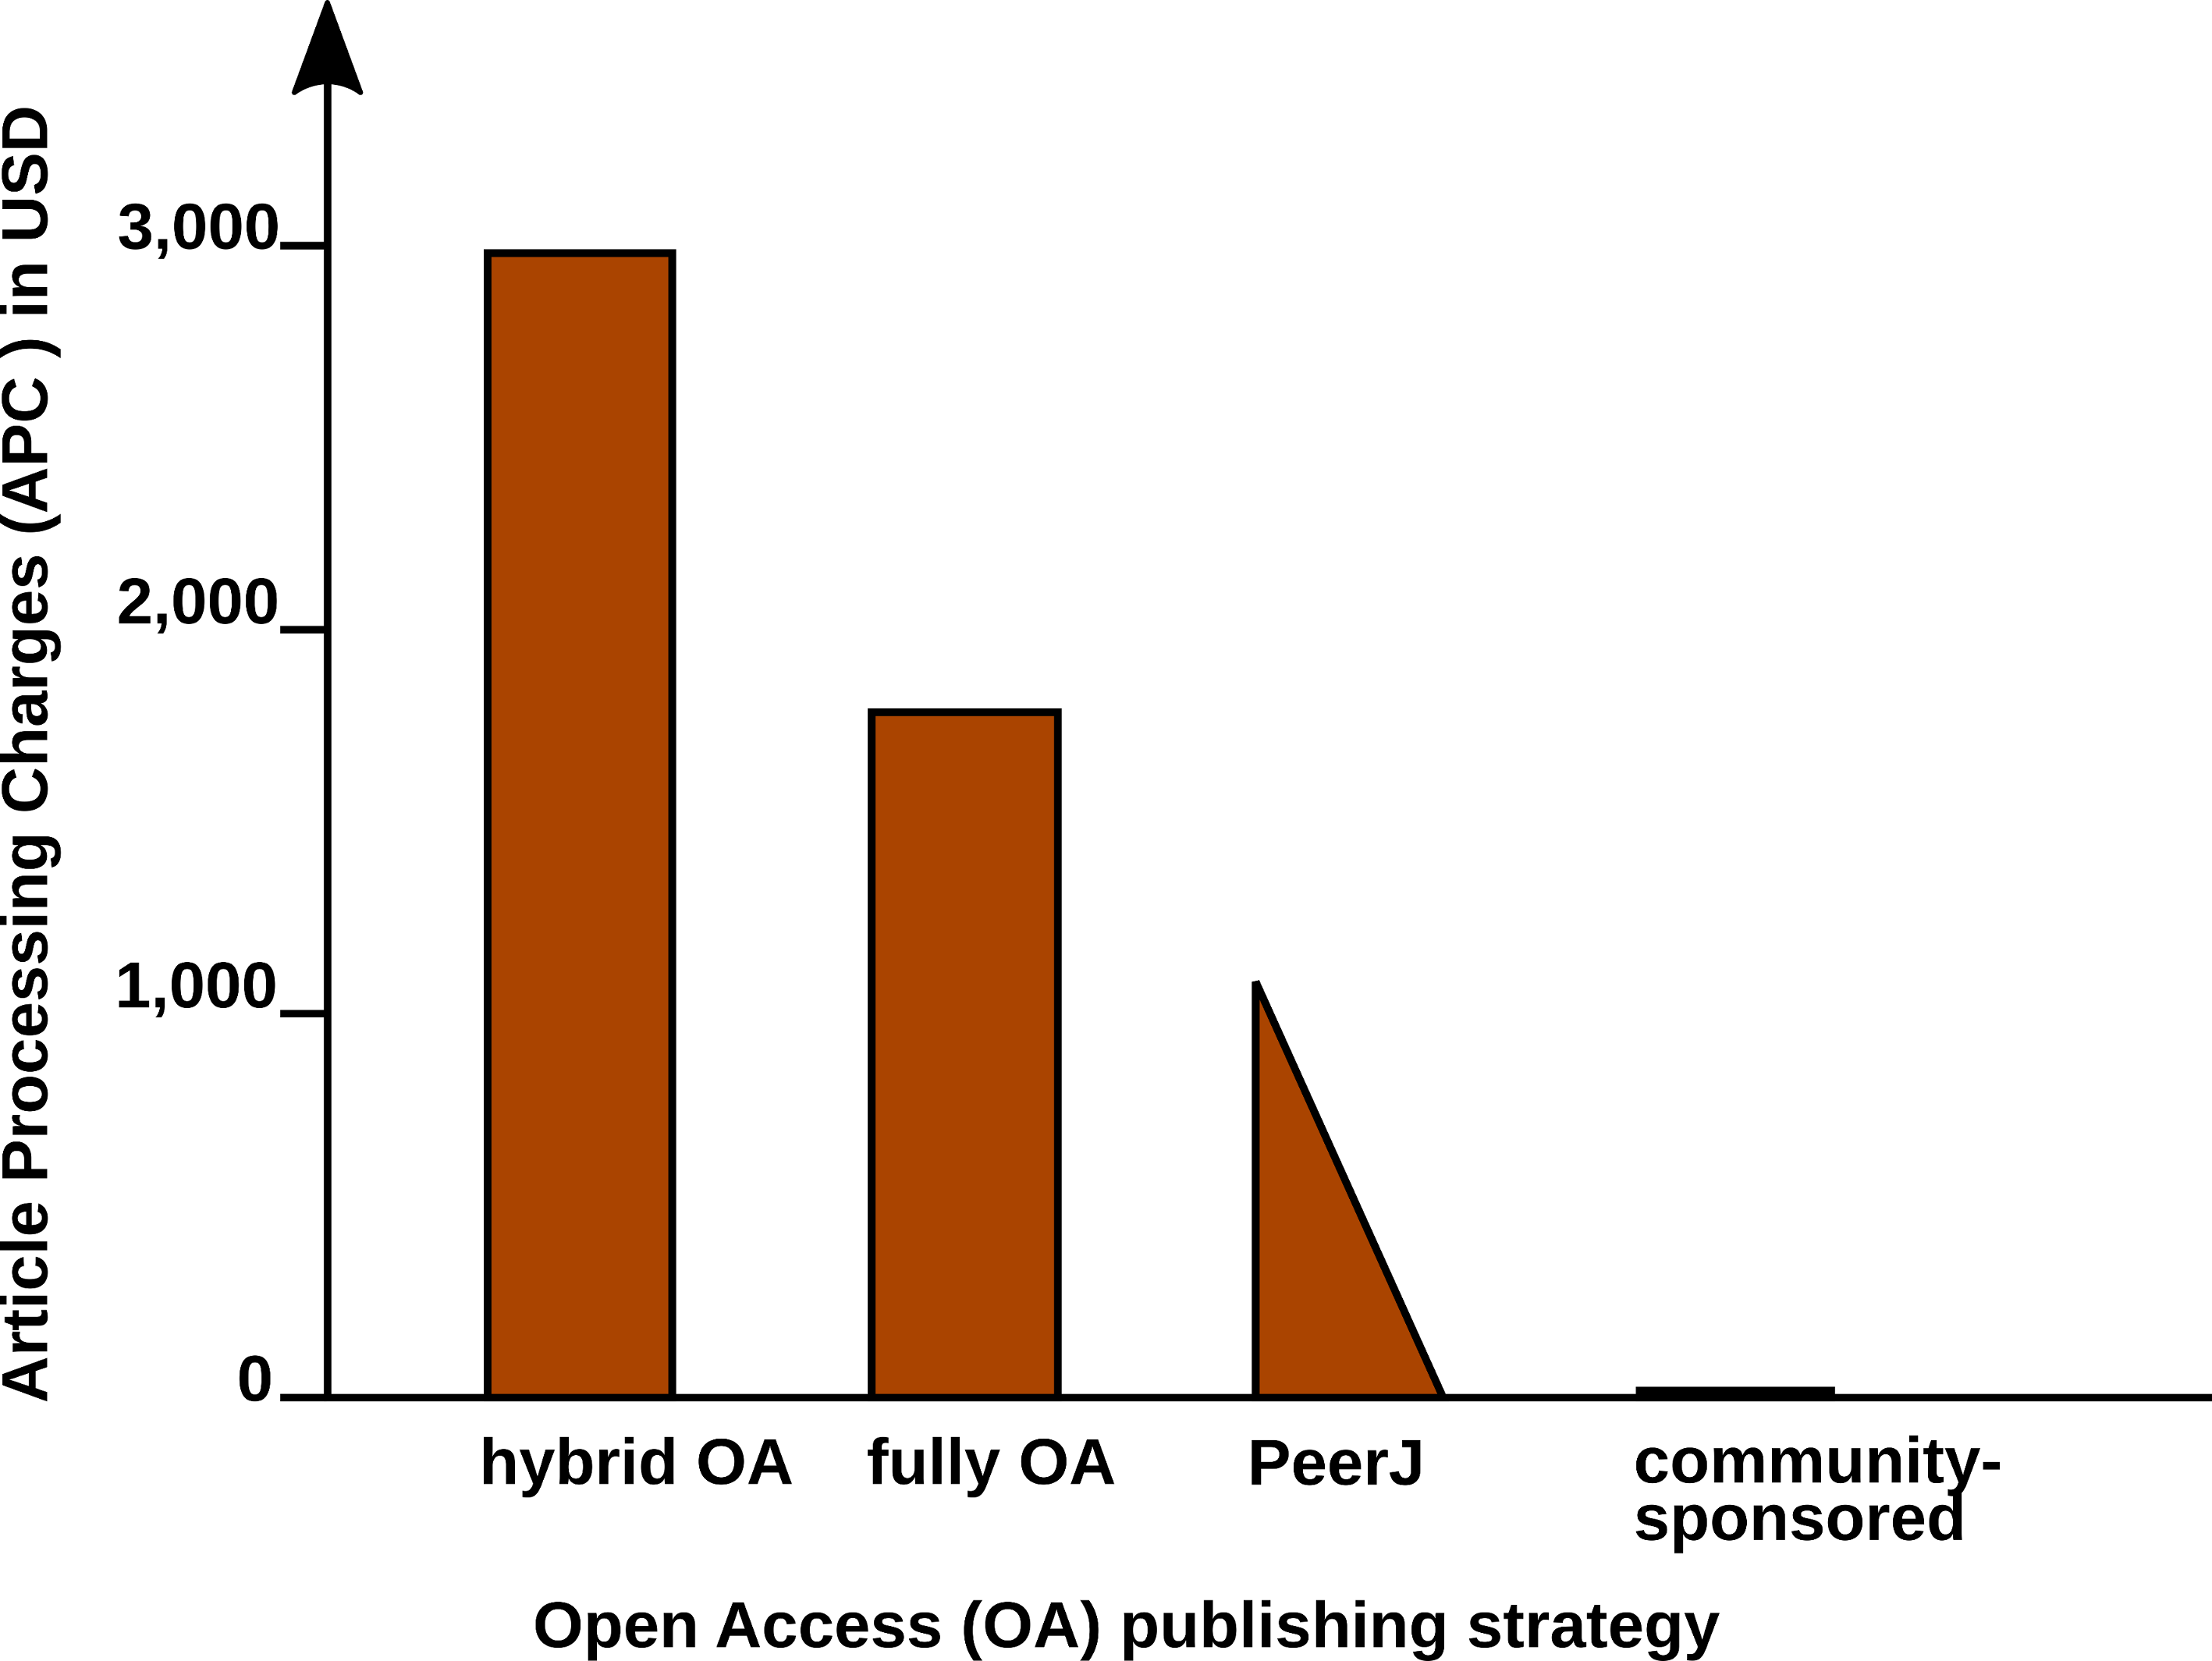
\includegraphics{fig-OA-strategies-APCs_small.png}
\caption{Article Processing Charge (APCs) that authors have to pay for
with different Open Access (OA) publishing models. Data from (Solomon \&
Björk, 2016) and journal web-pages.}
\end{figure}

In 2009, a study was carried out concerning the \emph{``Economic
Implications of Alternative Scholarly Publishing Models''}, which
demonstrates an overall societal benefit by using OA publishing model
(Houghton et al., 2009). In the same report, the real publication costs
are evaluated. The relative costs of an article for the publisher are
represented in \textbf{Fig. 2}.

\begin{figure}[htbp]
\centering
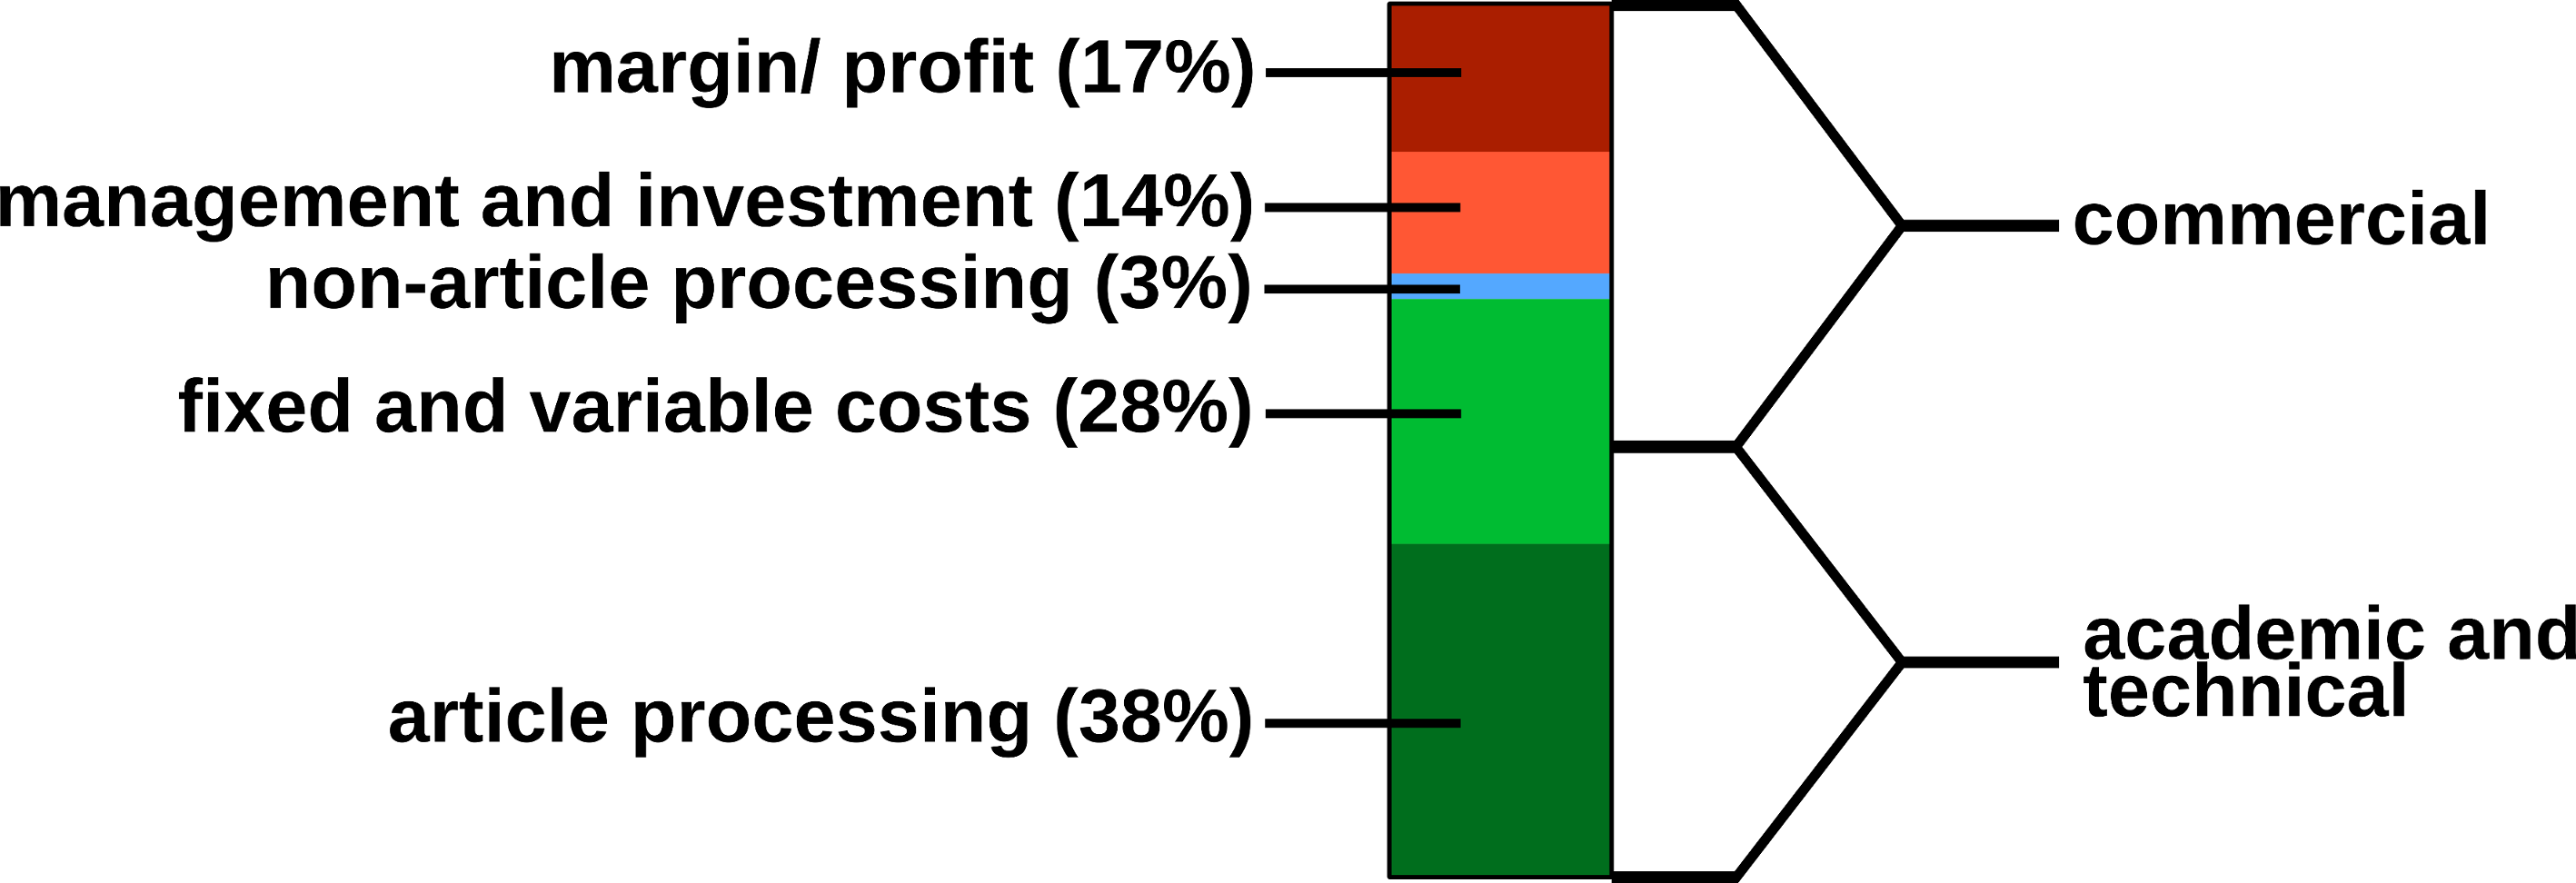
\includegraphics{fig-hybrid-publishing-costs_small.png}
\caption{Estimated publishing cost for a `hybrid' journal (conventional
with Open Access option). Data from (Houghton et al., 2009).}
\end{figure}

Conventional publishers justify their high subscription or APC prices
with the added value, e.g.~journalism (stated in the graphics as
`non-article processing'). But also stakeholder profits, which could be
as high as 50\%, must be considered, and are withdrawn from the science
budget (Van Noorden, 2013).

Generally, the production costs of an article could be roughly divided
into commercial and academic/ technical costs (\textbf{Fig. 2}). For
nonmarket production, the commercial costs such as margins/ profits,
management etc. can be drastically reduced. Hardware and services for
hosting an editorial system, such as Open Journal Systems of the Public
Knowledge Project (\url{https://pkp.sfu.ca/ojs/}) can be provided by
public institutions. Employed scholars can perform editor and reviewer
activities without additional cost for the journals. Nevertheless,
`article processing', which includes the manuscript handling during peer
review and production represents the most expensive part.

Therefore, we investigated a strategy for the efficient formatting of
scientific manuscripts.

\subsection{Current standard publishing
formats}\label{current-standard-publishing-formats}

Generally speaking, a scientific manuscript is composed of contents and
formatting. While the content, i.e.~text, figures, tables, citations
etc., may remain the same between different publishing forms and journal
styles, the formatting can be very different. Most publishers require
the formatting of submitted manuscripts in a certain format. Ignoring
this \textbf{Guide for Authors}, e.g.~by submitting a manuscript with a
different reference style, gives a negative impression with a journal's
editorial staff. Too carelessly prepared manuscripts can even provoke a
straight `desk-reject' (Volmer \& Stokes, 2016).

Currently DOC(X), LATEX and/ or PDF file formats are the most frequently
used formats for journal submission platforms. But even if the content
of a submitted manuscript might be accepted during the peer review `as
is', the format still needs to be adjusted to the particular publication
style in the production stage. For the electronic distribution and
archiving of scientific works, which is gaining more and more
importance, additional formats (EPUB, (X)HTML, JATS) need to be
generated. \textbf{Tab. 1} lists the file formats which are currently
the most relevant ones for scientific publishing.

Although the content elements of documents, such as title, author,
abstract, text, figures, tables, etc., remain the same, the syntax of
the file formats is rather different. \textbf{Tab. 2} demonstrates some
simple examples of differences in different markup languages.

Documents with the commonly used Office Open XML (DOCX Microsoft Word
files) and OpenDocument (ODT LibreOffice) file formats can be opened in
a standard text editor after unzipping. However, content and formatting
information is distributed into various folders and files. Practically
speaking, those file formats require the use of special word processing
software.

From a writer's perspective, the use of \emph{What You See Is What You
Get (WYSIWYG)} programs such as Microsoft Word, WPS Office or
LibreOffice might be convenient, because the formatting of the document
is directly visible. But the complicated syntax specifications often
result in problems when using different software versions and for
collaborative writing. Simple conversions between file formats can be
difficult or impossible. In a worst-case scenario, `old' files cannot be
opened any more for lack of compatible software.

In some parts of the scientific community therefore LATEX, a typesetting
program in plain text format, is very popular. With LATEX, documents
with highest typographic quality can be produced. However, the source
files are cluttered with LATEX commands and the source text can be
complicated to read. Causes of compilation errors in LATEX are sometimes
difficult to find. Therefore, LATEX is not very user friendly,
especially for casual writers or beginners.

\begin{longtable}[c]{@{}lllll@{}}
\caption{Current standard formats for scientific
publishing.}\tabularnewline
\toprule
\begin{minipage}[b]{0.06\columnwidth}\raggedright\strut
\textbf{Type}
\strut\end{minipage} &
\begin{minipage}[b]{0.18\columnwidth}\raggedright\strut
\textbf{Description}
\strut\end{minipage} &
\begin{minipage}[b]{0.13\columnwidth}\raggedright\strut
\textbf{Use}
\strut\end{minipage} &
\begin{minipage}[b]{0.09\columnwidth}\raggedright\strut
\textbf{Syntax}
\strut\end{minipage} &
\begin{minipage}[b]{0.40\columnwidth}\raggedright\strut
\textbf{Reference}
\strut\end{minipage}\tabularnewline
\midrule
\endfirsthead
\toprule
\begin{minipage}[b]{0.06\columnwidth}\raggedright\strut
\textbf{Type}
\strut\end{minipage} &
\begin{minipage}[b]{0.18\columnwidth}\raggedright\strut
\textbf{Description}
\strut\end{minipage} &
\begin{minipage}[b]{0.13\columnwidth}\raggedright\strut
\textbf{Use}
\strut\end{minipage} &
\begin{minipage}[b]{0.09\columnwidth}\raggedright\strut
\textbf{Syntax}
\strut\end{minipage} &
\begin{minipage}[b]{0.40\columnwidth}\raggedright\strut
\textbf{Reference}
\strut\end{minipage}\tabularnewline
\midrule
\endhead
\begin{minipage}[t]{0.06\columnwidth}\raggedright\strut
DOCX
\strut\end{minipage} &
\begin{minipage}[t]{0.18\columnwidth}\raggedright\strut
Office Open XML
\strut\end{minipage} &
\begin{minipage}[t]{0.13\columnwidth}\raggedright\strut
WYSIWYG editing
\strut\end{minipage} &
\begin{minipage}[t]{0.09\columnwidth}\raggedright\strut
XML, ZIP
\strut\end{minipage} &
\begin{minipage}[t]{0.40\columnwidth}\raggedright\strut
(Ngo, 2006)
\strut\end{minipage}\tabularnewline
\begin{minipage}[t]{0.06\columnwidth}\raggedright\strut
ODT
\strut\end{minipage} &
\begin{minipage}[t]{0.18\columnwidth}\raggedright\strut
OpenDocument
\strut\end{minipage} &
\begin{minipage}[t]{0.13\columnwidth}\raggedright\strut
WYSIWYG editing
\strut\end{minipage} &
\begin{minipage}[t]{0.09\columnwidth}\raggedright\strut
XML, ZIP
\strut\end{minipage} &
\begin{minipage}[t]{0.40\columnwidth}\raggedright\strut
(Brauer et al., 2005)
\strut\end{minipage}\tabularnewline
\begin{minipage}[t]{0.06\columnwidth}\raggedright\strut
PDF
\strut\end{minipage} &
\begin{minipage}[t]{0.18\columnwidth}\raggedright\strut
portable document
\strut\end{minipage} &
\begin{minipage}[t]{0.13\columnwidth}\raggedright\strut
print replacement
\strut\end{minipage} &
\begin{minipage}[t]{0.09\columnwidth}\raggedright\strut
PDF
\strut\end{minipage} &
\begin{minipage}[t]{0.40\columnwidth}\raggedright\strut
(International Organization for Standardization, 2013)
\strut\end{minipage}\tabularnewline
\begin{minipage}[t]{0.06\columnwidth}\raggedright\strut
EPUB
\strut\end{minipage} &
\begin{minipage}[t]{0.18\columnwidth}\raggedright\strut
electronic publishing
\strut\end{minipage} &
\begin{minipage}[t]{0.13\columnwidth}\raggedright\strut
e-books
\strut\end{minipage} &
\begin{minipage}[t]{0.09\columnwidth}\raggedright\strut
HTML5, ZIP
\strut\end{minipage} &
\begin{minipage}[t]{0.40\columnwidth}\raggedright\strut
(Eikebrokk, Dahl \& Kessel, 2014)
\strut\end{minipage}\tabularnewline
\begin{minipage}[t]{0.06\columnwidth}\raggedright\strut
JATS
\strut\end{minipage} &
\begin{minipage}[t]{0.18\columnwidth}\raggedright\strut
journal article tag suite
\strut\end{minipage} &
\begin{minipage}[t]{0.13\columnwidth}\raggedright\strut
journal publishing
\strut\end{minipage} &
\begin{minipage}[t]{0.09\columnwidth}\raggedright\strut
XML
\strut\end{minipage} &
\begin{minipage}[t]{0.40\columnwidth}\raggedright\strut
(National Information Standards Organization, 2012)
\strut\end{minipage}\tabularnewline
\begin{minipage}[t]{0.06\columnwidth}\raggedright\strut
LATEX
\strut\end{minipage} &
\begin{minipage}[t]{0.18\columnwidth}\raggedright\strut
typesetting system
\strut\end{minipage} &
\begin{minipage}[t]{0.13\columnwidth}\raggedright\strut
high-quality print
\strut\end{minipage} &
\begin{minipage}[t]{0.09\columnwidth}\raggedright\strut
TEX
\strut\end{minipage} &
\begin{minipage}[t]{0.40\columnwidth}\raggedright\strut
(Lamport, 1994)
\strut\end{minipage}\tabularnewline
\begin{minipage}[t]{0.06\columnwidth}\raggedright\strut
HTML
\strut\end{minipage} &
\begin{minipage}[t]{0.18\columnwidth}\raggedright\strut
hypertext markup
\strut\end{minipage} &
\begin{minipage}[t]{0.13\columnwidth}\raggedright\strut
websites
\strut\end{minipage} &
\begin{minipage}[t]{0.09\columnwidth}\raggedright\strut
(X)HTML
\strut\end{minipage} &
\begin{minipage}[t]{0.40\columnwidth}\raggedright\strut
(Raggett et al., 1999; Hickson et al., 2014)
\strut\end{minipage}\tabularnewline
\begin{minipage}[t]{0.06\columnwidth}\raggedright\strut
MD
\strut\end{minipage} &
\begin{minipage}[t]{0.18\columnwidth}\raggedright\strut
Markdown
\strut\end{minipage} &
\begin{minipage}[t]{0.13\columnwidth}\raggedright\strut
lightweight markup
\strut\end{minipage} &
\begin{minipage}[t]{0.09\columnwidth}\raggedright\strut
plain text MD
\strut\end{minipage} &
\begin{minipage}[t]{0.40\columnwidth}\raggedright\strut
(Ovadia, 2014; Leonard, 2016)
\strut\end{minipage}\tabularnewline
\bottomrule
\end{longtable}

\begin{longtable}[c]{@{}llll@{}}
\caption{Examples for formatting elements and their implementations in
different markup languages.}\tabularnewline
\toprule
\begin{minipage}[b]{0.11\columnwidth}\raggedright\strut
\textbf{Element}
\strut\end{minipage} &
\begin{minipage}[b]{0.17\columnwidth}\raggedright\strut
\textbf{Markdown}
\strut\end{minipage} &
\begin{minipage}[b]{0.33\columnwidth}\raggedright\strut
\textbf{LATEX}
\strut\end{minipage} &
\begin{minipage}[b]{0.27\columnwidth}\raggedright\strut
\textbf{HTML}
\strut\end{minipage}\tabularnewline
\midrule
\endfirsthead
\toprule
\begin{minipage}[b]{0.11\columnwidth}\raggedright\strut
\textbf{Element}
\strut\end{minipage} &
\begin{minipage}[b]{0.17\columnwidth}\raggedright\strut
\textbf{Markdown}
\strut\end{minipage} &
\begin{minipage}[b]{0.33\columnwidth}\raggedright\strut
\textbf{LATEX}
\strut\end{minipage} &
\begin{minipage}[b]{0.27\columnwidth}\raggedright\strut
\textbf{HTML}
\strut\end{minipage}\tabularnewline
\midrule
\endhead
\begin{minipage}[t]{0.11\columnwidth}\raggedright\strut
\textbf{structure}
\strut\end{minipage} &
\begin{minipage}[t]{0.17\columnwidth}\raggedright\strut
\strut\end{minipage} &
\begin{minipage}[t]{0.33\columnwidth}\raggedright\strut
\strut\end{minipage}\tabularnewline
\begin{minipage}[t]{0.11\columnwidth}\raggedright\strut
section
\strut\end{minipage} &
\begin{minipage}[t]{0.17\columnwidth}\raggedright\strut
\texttt{\#\ Intro}
\strut\end{minipage} &
\begin{minipage}[t]{0.33\columnwidth}\raggedright\strut
\texttt{\textbackslash{}section\{Intro\}}
\strut\end{minipage} &
\begin{minipage}[t]{0.27\columnwidth}\raggedright\strut
\texttt{\textless{}h1\textgreater{}\textless{}Intro\textgreater{}\textless{}/h1\textgreater{}}
\strut\end{minipage}\tabularnewline
\begin{minipage}[t]{0.11\columnwidth}\raggedright\strut
subsection
\strut\end{minipage} &
\begin{minipage}[t]{0.17\columnwidth}\raggedright\strut
\texttt{\#\#\ History}
\strut\end{minipage} &
\begin{minipage}[t]{0.33\columnwidth}\raggedright\strut
\texttt{\textbackslash{}subsection\{History\}}
\strut\end{minipage} &
\begin{minipage}[t]{0.27\columnwidth}\raggedright\strut
\texttt{\textless{}h2\textgreater{}\textless{}History\textgreater{}\textless{}/h2\textgreater{}}
\strut\end{minipage}\tabularnewline
\begin{minipage}[t]{0.11\columnwidth}\raggedright\strut
\textbf{text style}
\strut\end{minipage} &
\begin{minipage}[t]{0.17\columnwidth}\raggedright\strut
\strut\end{minipage} &
\begin{minipage}[t]{0.33\columnwidth}\raggedright\strut
\strut\end{minipage}\tabularnewline
\begin{minipage}[t]{0.11\columnwidth}\raggedright\strut
bold
\strut\end{minipage} &
\begin{minipage}[t]{0.17\columnwidth}\raggedright\strut
\texttt{**text**}
\strut\end{minipage} &
\begin{minipage}[t]{0.33\columnwidth}\raggedright\strut
\texttt{\textbackslash{}textbf\{text\}}
\strut\end{minipage} &
\begin{minipage}[t]{0.27\columnwidth}\raggedright\strut
\texttt{\textless{}b\textgreater{}text\textless{}/b\textgreater{}}
\strut\end{minipage}\tabularnewline
\begin{minipage}[t]{0.11\columnwidth}\raggedright\strut
italics
\strut\end{minipage} &
\begin{minipage}[t]{0.17\columnwidth}\raggedright\strut
\texttt{*text*}
\strut\end{minipage} &
\begin{minipage}[t]{0.33\columnwidth}\raggedright\strut
\texttt{\textbackslash{}textit\{text\}}
\strut\end{minipage} &
\begin{minipage}[t]{0.27\columnwidth}\raggedright\strut
\texttt{\textless{}i\textgreater{}text\textless{}/i\textgreater{}}
\strut\end{minipage}\tabularnewline
\begin{minipage}[t]{0.11\columnwidth}\raggedright\strut
\textbf{links}
\strut\end{minipage} &
\begin{minipage}[t]{0.17\columnwidth}\raggedright\strut
\strut\end{minipage} &
\begin{minipage}[t]{0.33\columnwidth}\raggedright\strut
\strut\end{minipage}\tabularnewline
\begin{minipage}[t]{0.11\columnwidth}\raggedright\strut
HTTP link
\strut\end{minipage} &
\begin{minipage}[t]{0.17\columnwidth}\raggedright\strut
\texttt{\textless{}https://\ arxiv.org\textgreater{}}
\strut\end{minipage} &
\begin{minipage}[t]{0.33\columnwidth}\raggedright\strut
\texttt{\textbackslash{}usepackage\{url\}\ \textbackslash{}url\{https://arxiv.org\}}
\strut\end{minipage} &
\begin{minipage}[t]{0.27\columnwidth}\raggedright\strut
\texttt{\textless{}a\ href="https://\ arxiv.org"\textgreater{}\textless{}/a\textgreater{}}
\strut\end{minipage}\tabularnewline
\bottomrule
\end{longtable}

In academic publishing, it is additionally desirable to create different
output formats from the same source text:

\begin{itemize}
\tightlist
\item
  For the publishing of a book, with a print version in PDF and an
  electronic version in EPUB.
\item
  For the distribution of a seminar script, with an online version in
  HTML and a print version in PDF.
\item
  For submitting a journal manuscript for peer-review in DOCX, as well
  as a preprint version with another journal style in PDF.
\item
  For archiving and exchanging article data using the Journal Article
  Tag Suite (JATS) (National Information Standards Organization, 2012),
  a standardized format developed by the NLM.
\end{itemize}

Some of the tasks can be performed e.g.~with LATEX, but an integrated
solution remains a challenge. Several programs for the conversion
between documents formats exist, such as the e-book library program
calibre \url{http://calibre-ebook.com/}. But the results of such
conversions are often not satisfactory and require substantial manual
corrections.

Therefore, we were looking for a solution that enables the creation of
scientific manuscripts in a simple format, with the subsequent
generation of multiple output formats. The need for hybrid publishing
has been recognized outside of science (Kielhorn, 2011; DPT Collective,
2015), but the requirements specific to scientific publishing have not
been addressed so far. Therefore, we investigated the possibility to
generate multiple publication formats from a simple manuscript source
file.

\section{Concepts of markdown and
pandoc}\label{concepts-of-markdown-and-pandoc}

Markdown was originally developed by John Gruber in collaboration with
Aaron Swartz, with the goal to simplify the writing of HTML documents
\url{http://daringfireball.net/projects/markdown/}. Instead of coding a
file in HTML syntax, the content of a document is written in plain text
and annotated with simple tags which define the formatting.
Subsequently, the Markdown (MD) files are parsed to generate the final
HTML document. With this concept, the source file remains easily
readable and the author can focus on the contents rather than
formatting. Despite its original focus on the web, the MD format has
been proven to be well suited for academic writing (Ovadia, 2014). In
particular, pandoc-flavored MD (\url{http://pandoc.org/}) adds several
extensions which facilitate the authoring of academic documents and
their conversion into multiple output formats. \textbf{Tab. 2}
demonstrates the simplicity of MD compared to other markup languages.
\textbf{Fig. 3} illustrates the generation of various formatted
documents from a manuscript in pandoc MD. Some relevant functions for
scientific texts are explained below in more detail.

\begin{figure}[htbp]
\centering
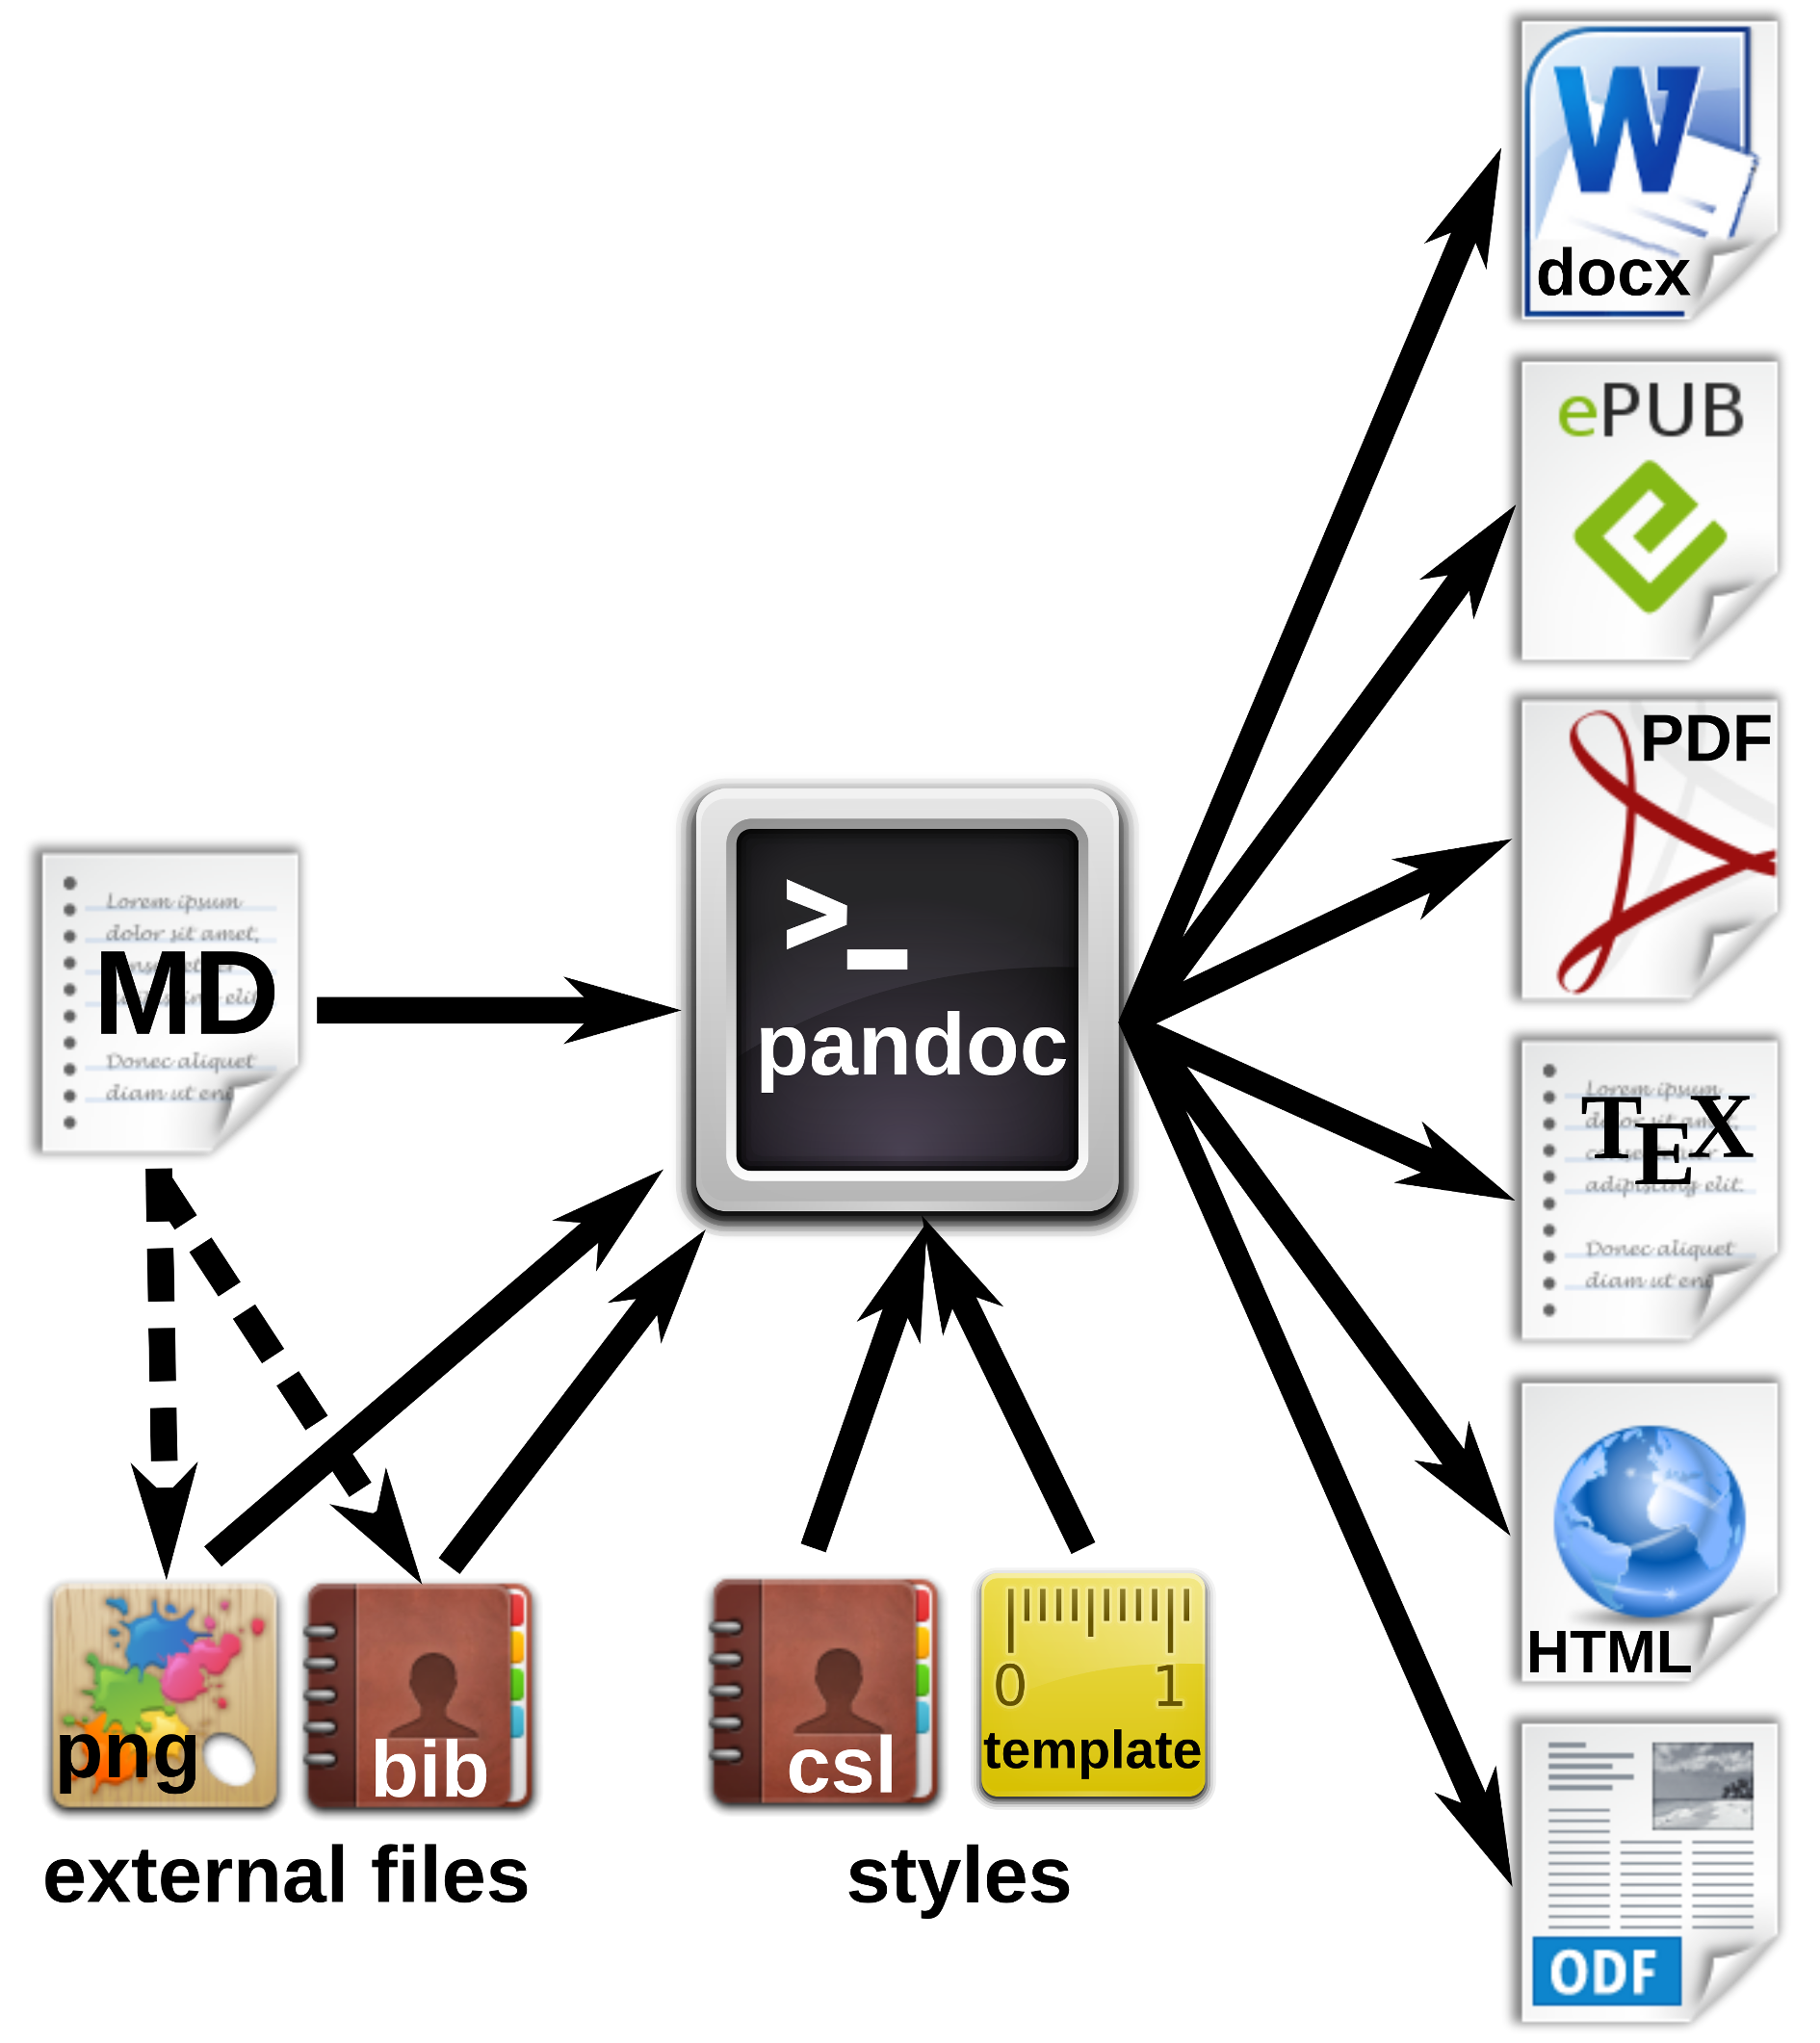
\includegraphics{fig-pandoc-workflow_small.png}
\caption{Workfow for the generation of multiple document formats with
pandoc. The markdown (MD) file contains the manuscript text with
formatting tags, and can also refer to external files such as images or
reference databases. The pandoc processor converts the MD file to the
desired output formats. Documents, citations etc. can be defined in
style files or templates.}
\end{figure}

\section{Markdown editors and online
editing}\label{markdown-editors-and-online-editing}

The usability of a text editor is important for the author, either
writing alone or with several co-authors. In this section we present
software and strategies for different scenarios. \textbf{Fig. 4}
summarizes various options for local or networked editing of MD files.

\begin{figure}[htbp]
\centering
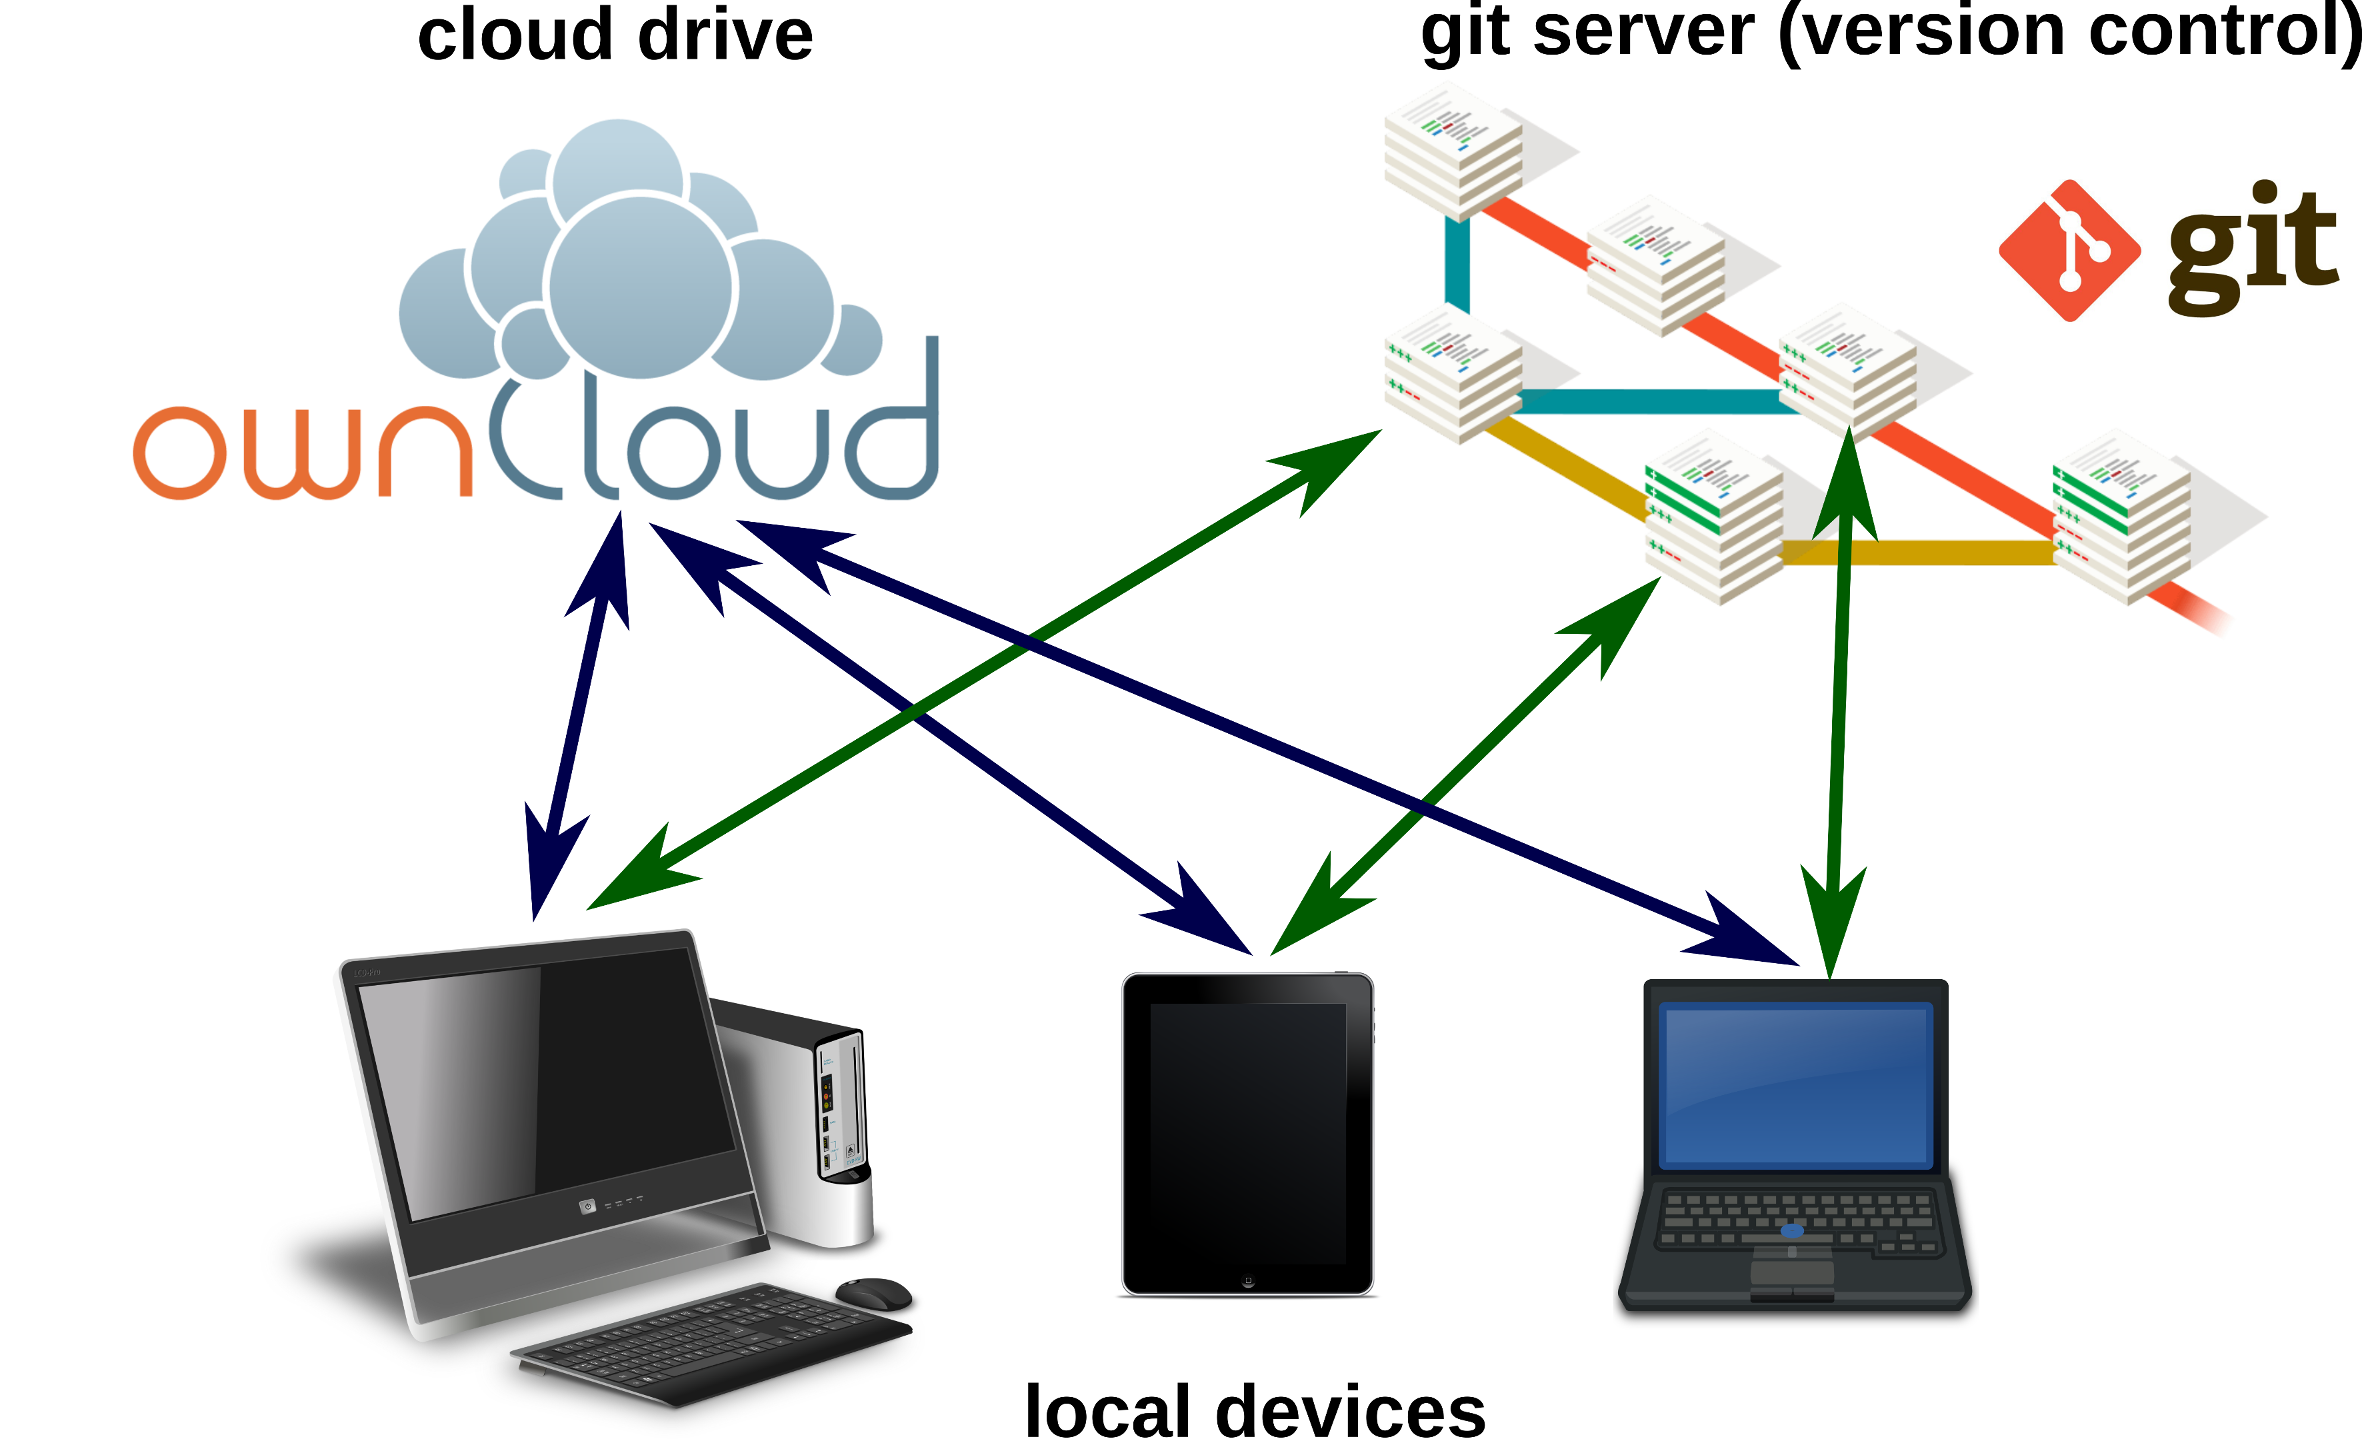
\includegraphics{fig-editing-options_small.png}
\caption{Markdown files can be edited on local devices or on cloud
drives. A local or remote git repository enables advanced advanced
version control.}
\end{figure}

\subsection{Markdown editors}\label{markdown-editors}

Due to MD's simple syntax, basically any text editor is suitable for
editing markdown files. The formatting tags are written in plain text
and are easy to remember. Therefore, the author is not distracted by
looking around for layout options with the mouse. For several popular
text editors, such as vim (\url{http://www.vim.org/}), GNU Emacs
(\url{https://www.gnu.org/software/emacs/}), atom
(\url{https://atom.io/}) or geany (\url{http://www.geany.org/}), plugins
provide additional functionality for markdown editing, e.g.~syntax
highlighting, command helpers, live preview or structure browsing.

Various dedicated markdown editors have been published as well. Many of
those are cross-platform compatible, such as Abricotine
(\url{http://abricotine.brrd.fr/}), ghostwriter
(\url{https://github.com/wereturtle/ghostwriter}) and CuteMarkEd
(\url{https://cloose.github.io/CuteMarkEd/}).

The lightweight format is also ideal for writing on mobile devices.
Numerous applications are available on the App stores for Android and
iOS systems. The programs Swype and Dragon
(\url{http://www.nuance.com/}) facilitate the input of text on such
devices by guessing words from gestures and speech recognition
(dictation).

\textbf{Fig. 5.} shows the editing of a markdown file, using the
cross-platform editor Atom with several markdown plugins.

\begin{figure}[htbp]
\centering
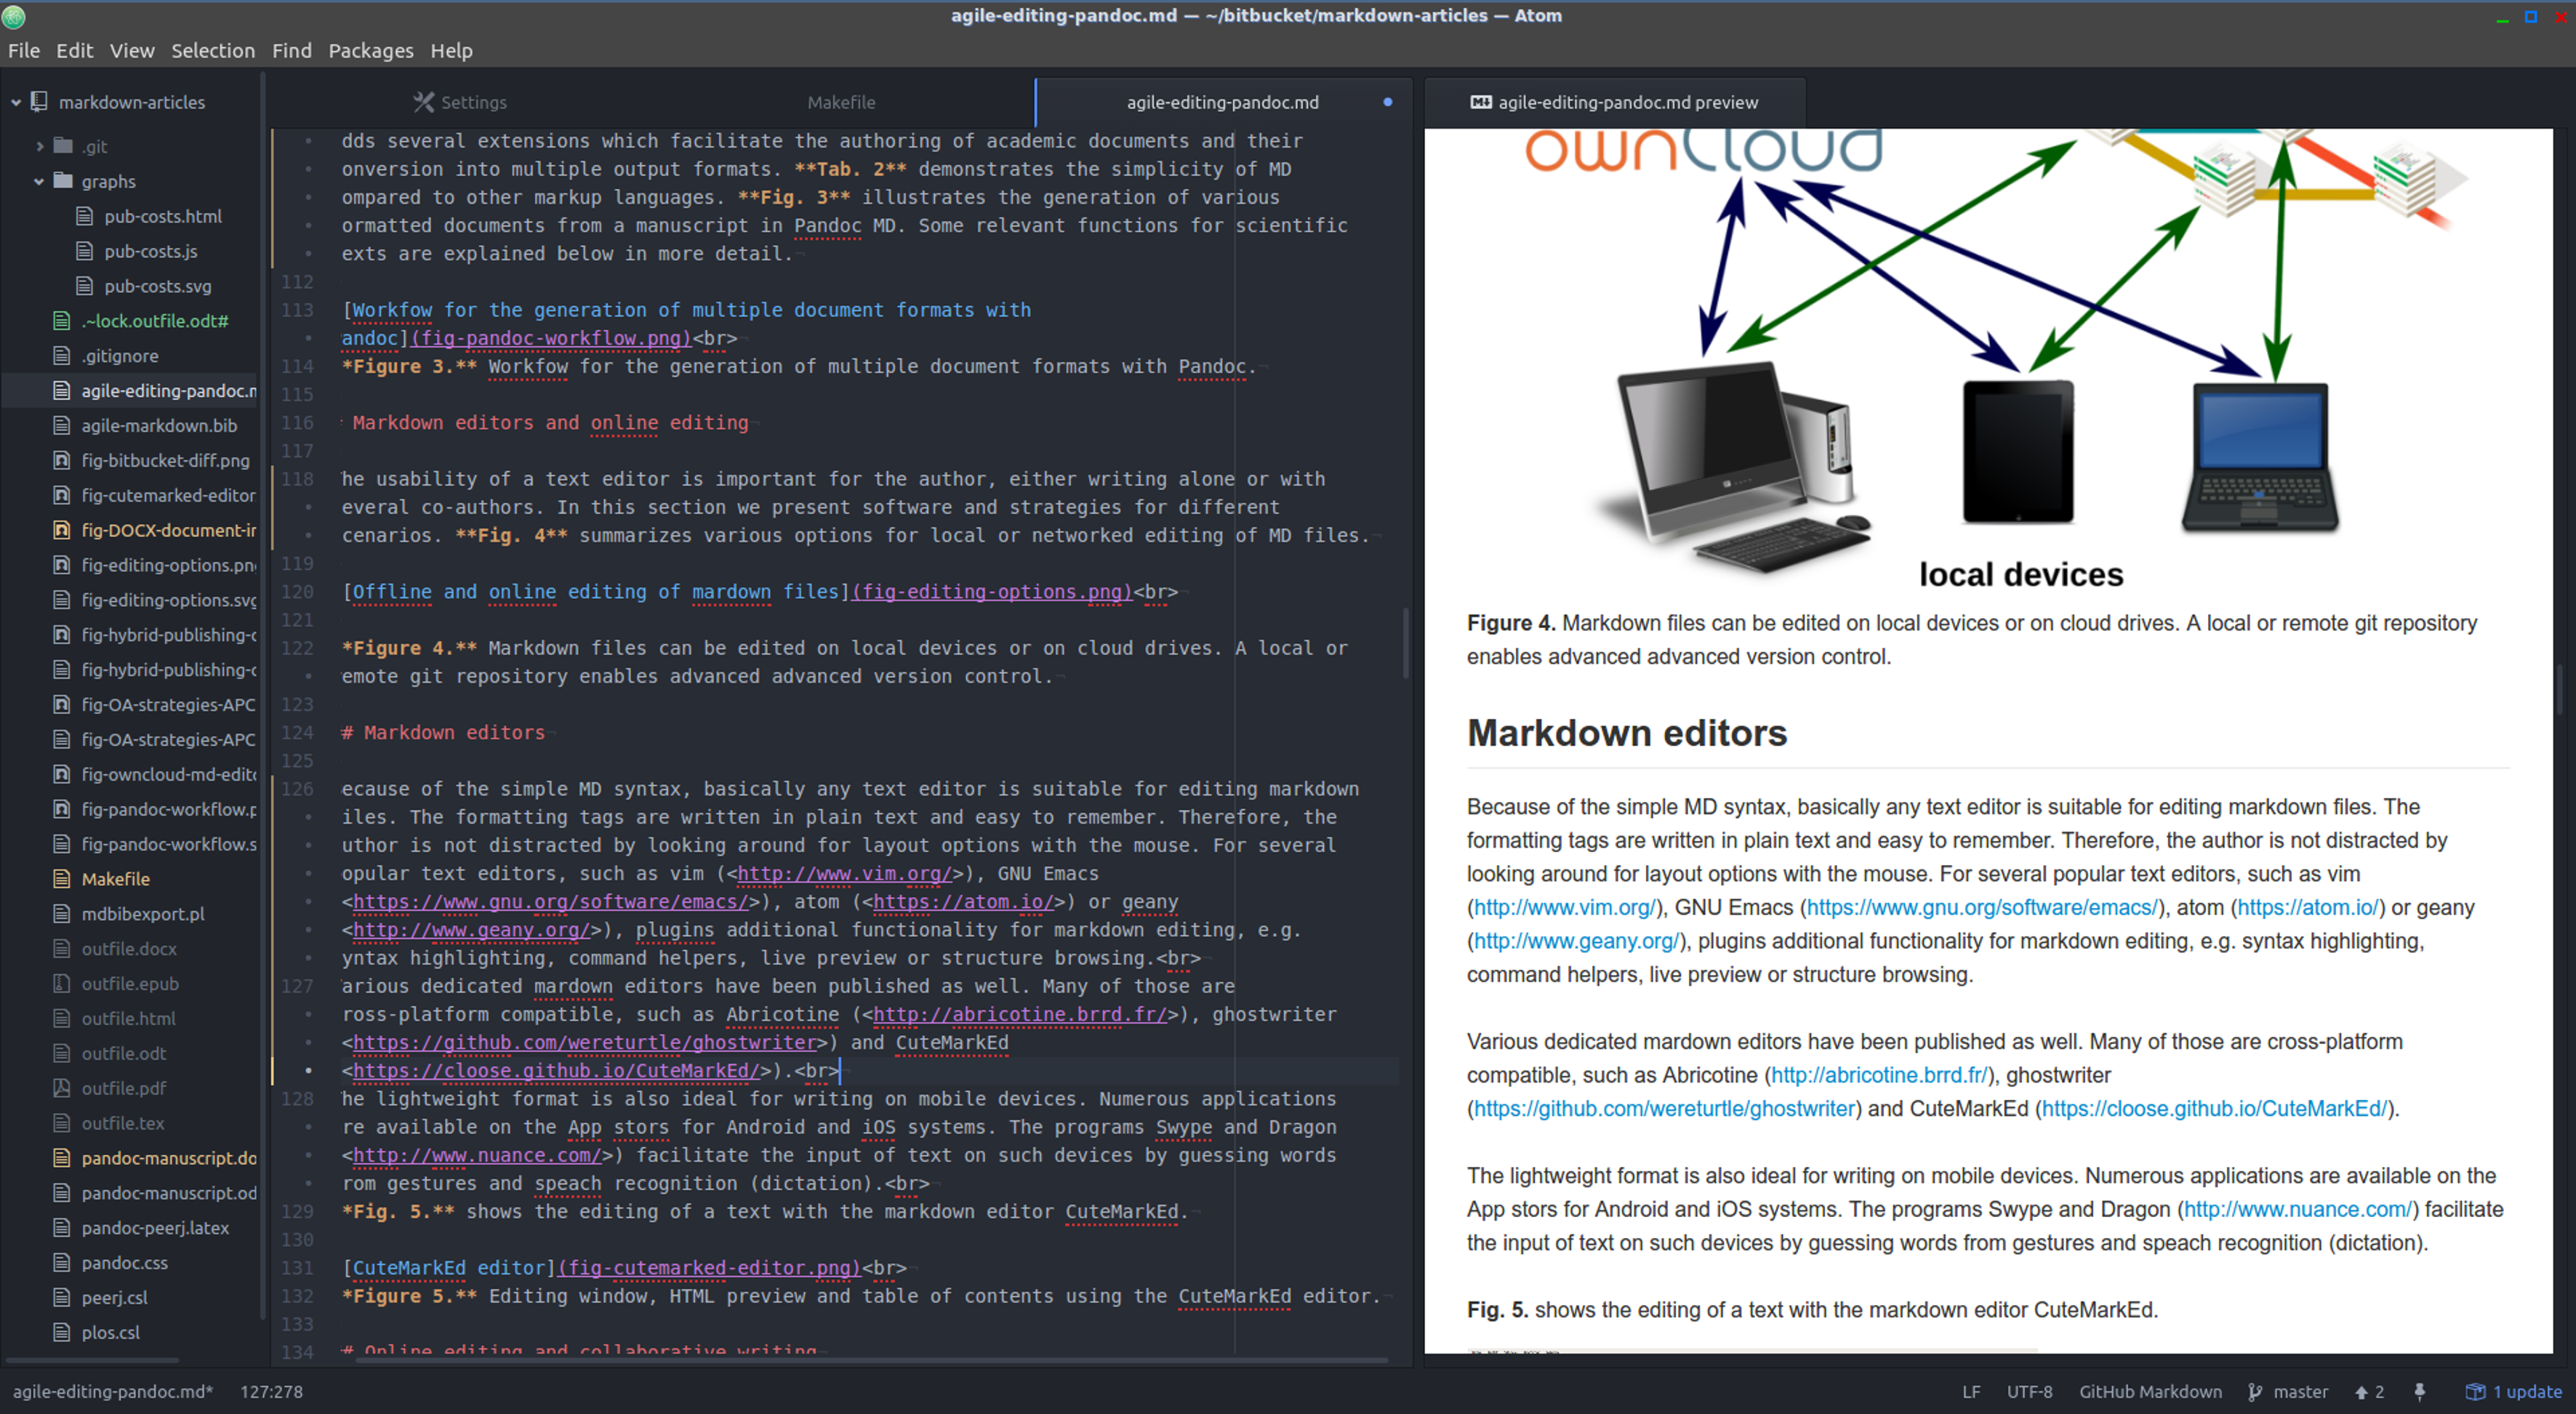
\includegraphics{fig-atom-editor.png}
\caption{Document directory tree, editing window and HTML preview using
the Atom editor.}
\end{figure}

\subsection{Online editing and collaborative
writing}\label{online-editing-and-collaborative-writing}

Storing manuscripts on network drives (\emph{The Cloud}) has become
popular for several reasons:

\begin{itemize}
\tightlist
\item
  Protection against data loss.
\item
  Synchronization of documents between several devices.
\item
  Collaborative editing options.
\end{itemize}

Markdown files on a Google Drive (\url{https://drive.google.com}) for
instance can be edited online with StackEdit
(\url{https://stackedit.io}). \textbf{Fig. 6} demonstrates the online
editing of a markdown file on an ownCloud (\url{https://owncloud.com/})
installation. OwnCloud is an Open Source software platform, which allows
the set-up of a file server on personal webspace. The functionality of
an ownCloud installation can be enhanced by installing plugins.

\begin{figure}[htbp]
\centering
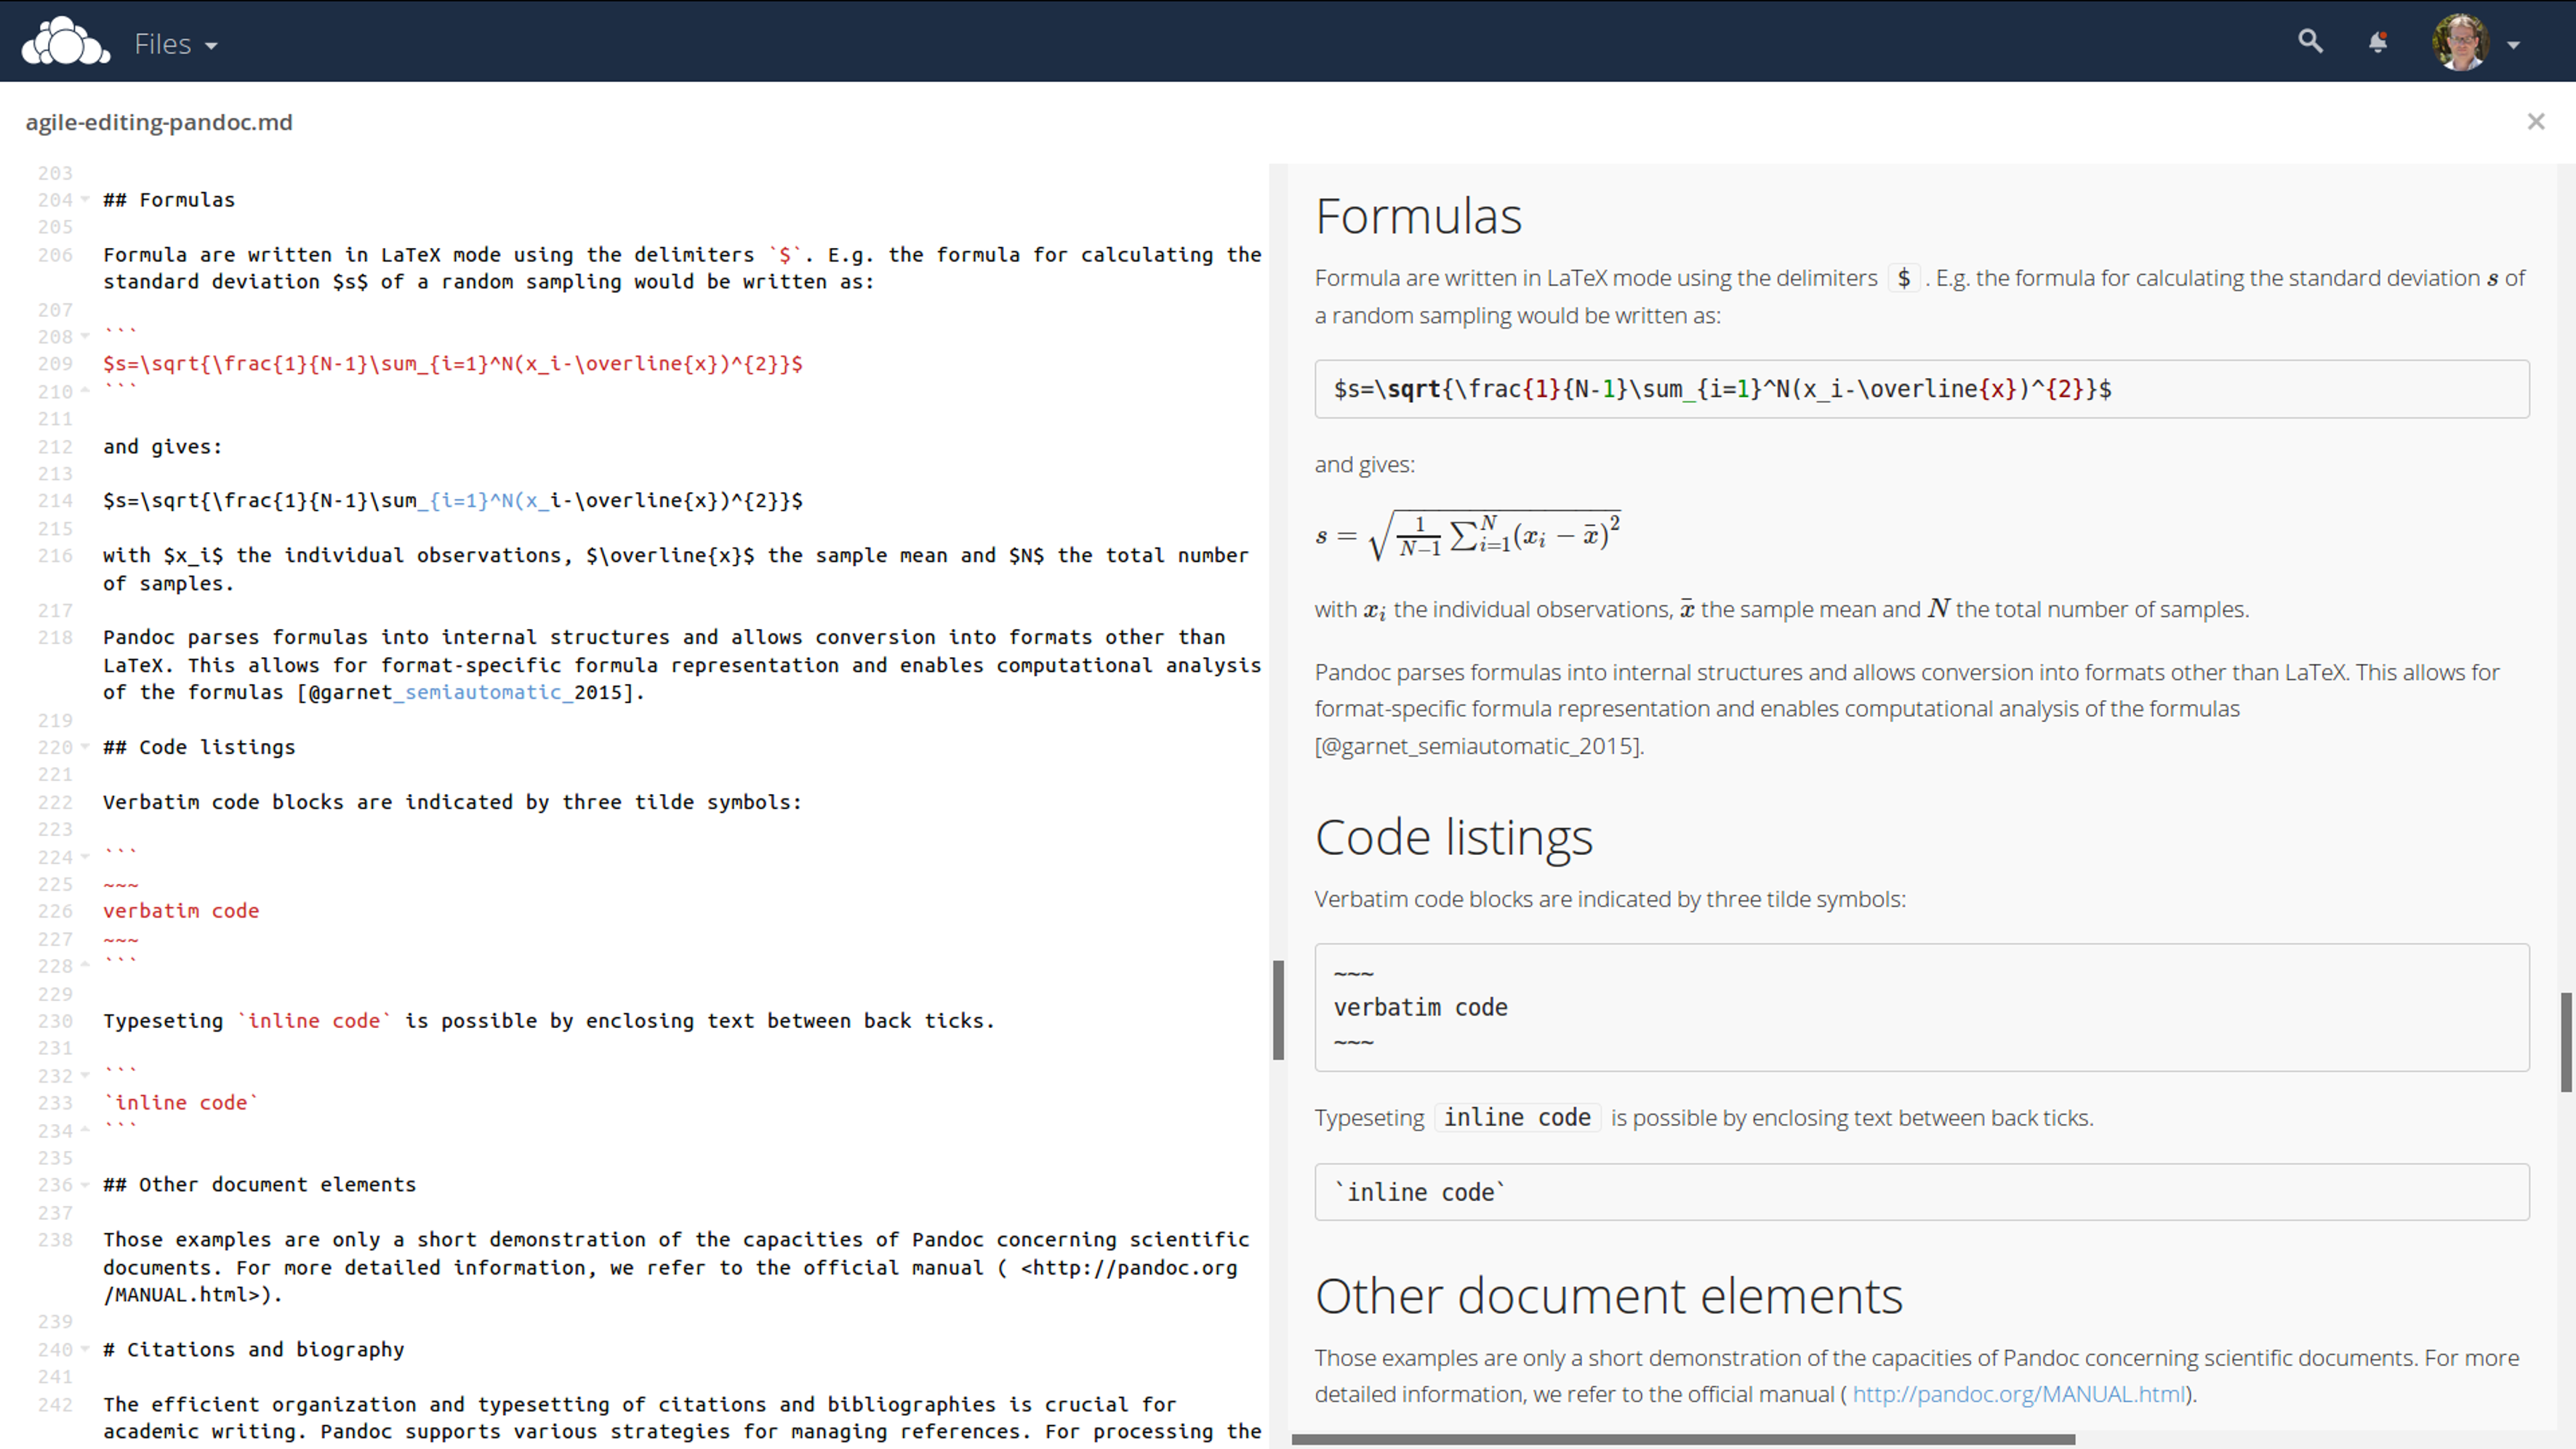
\includegraphics{fig-owncloud-md-editor.png}
\caption{Direct online editing of this manuscript with live preview
using the ownCloud Markdown Editor plugin by Robin Appelman.}
\end{figure}

Even mathematical formulas are rendered correctly in the HTML live
preview window of the ownCloud markdown plugin (\textbf{Fig. 6} ).

The collaboration and authoring platform Authorea
(\url{https://www.authorea.com/}) also supports markdown as one of
multiple possible input formats. This can be beneficial for
collaborations in which one or more authors are not familiar with
markdown syntax.

\subsection{Document versioning and change
control}\label{document-versioning-and-change-control}

Programmers, especially when working in distributed teams, rely on
version control systems to manage changes of code. Currently, Git
(\url{https://git-scm.com/}), which is also used e.g.~for the
development of the Linux kernel, is one of the most employed software
solutions for versioning. Git allows the parallel work of collaborators
and has an efficient merging and conflict resolution system. A Git
repository may be used by a single local author to keep track of
changes, or by a team with a remote repository, e.g.~on github
(\url{https://github.com/}) or bitbucket (\url{https://bitbucket.org/}).
Because of the plain text format of markdown, Git can be used for
version control and distributed writing. For the writing of the present
article, the co-authors (Germany and Mexico) used a remote Git
repository on bitbucket. The plain text syntax of markdown facilitates
the visualization of differences of document versions, as shown in
\textbf{Fig. 7}.

\begin{figure}[htbp]
\centering
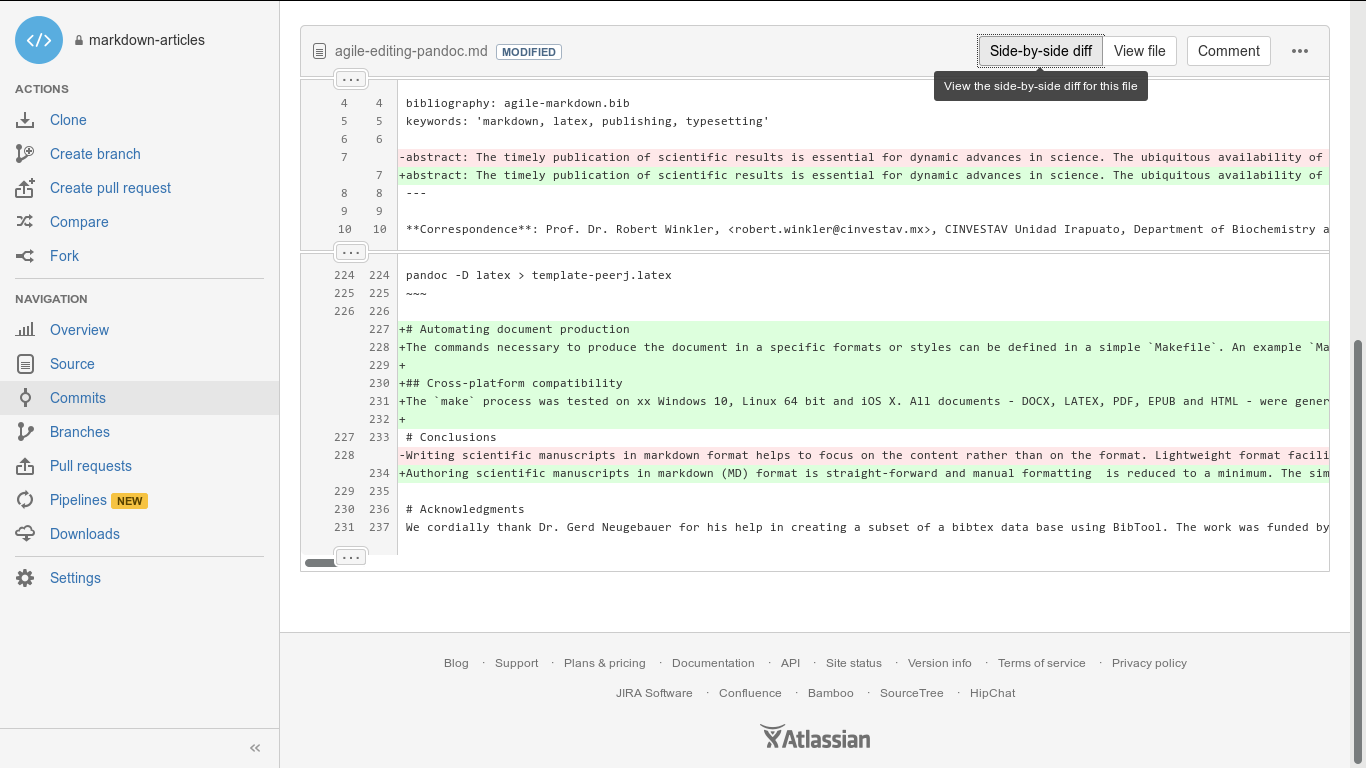
\includegraphics{fig-bitbucket-diff.png}
\caption{Version control and collaborative editing using a git
repository on bitbucket.}
\end{figure}

\section{Pandoc markdown for scientific
texts}\label{pandoc-markdown-for-scientific-texts}

In the following section, we demonstrate the potential for typesetting
scientific manuscripts with pandoc using examples for typical document
elements, such as tables, figures, formulas, code listings and
references. A brief introduction is given by Dominici (2014). The
complete Pandoc User's Manual is available at
\url{http://pandoc.org/MANUAL.html}.

\subsection{Tables}\label{tables}

There are several options to write tables in markdown. The most flexible
alternative - which was also used for this article - are pipe tables.
The contents of different cells are separated by pipe symbols
(\texttt{\textbar{}}):

\begin{verbatim}
Left | Center | Right | Default
:-----|:------:|------:|---------
 LLL  | CCC    | RRR   | DDD
\end{verbatim}

gives

\begin{longtable}[c]{@{}lcrl@{}}
\toprule
Left & Center & Right & Default\tabularnewline
\midrule
\endhead
LLL & CCC & RRR & DDD\tabularnewline
\bottomrule
\end{longtable}

The headings and the alignment of the cells are given in the first two
lines. The cell width is variable. The pandoc parameter
\texttt{-\/-columns=NUM} can be used to define the length of lines in
characters. If contents do not fit, they will be wrapped.

Complex tables, e.g.~tables featuring multiple headers or those
containing cells spanning multiple rows or columns, are currently not
representable in markdown format. However, it is possible to embed LATEX
and HTML tables into the document. These format-specific tables will
only be included in the output if a document of the respective format is
produced. This is method can be extended to apply any kind of
format-specific typographic functionality which would otherwise be
unavailable in markdown syntax.

\subsection{Figures and images}\label{figures-and-images}

Images are inserted as follows:

\begin{verbatim}
![alt text](image location/ name)
\end{verbatim}

e.g.

\begin{verbatim}
![Publishing costs](fig-hybrid-publishing-costs.png)
\end{verbatim}

The \emph{alt text} is used e.g.~in HTML output. Image dimensions can be
defined in braces:

\begin{verbatim}
![](fig-hybrid-publishing-costs.png)
\end{verbatim}

As well, an identifier for the figure can be defined with \texttt{\#},
resulting e.g.~in the image attributes
\texttt{\{\#figure1\ height=30\%\}}.

A paragraph containing only an image is interpreted as a figure. The
\emph{alt text} is then output as the figure's caption.

\subsection{Symbols}\label{symbols}

Scientific texts often require special characters, e.g.~Greek letters,
mathematical and physical symbols etc.

The UTF-8 standard, developed and maintained by \emph{Unicode
Consortium}, enables the use of characters across languages and computer
platforms. The encoding is defined as RFC document 3629 of the Network
Working group (Yergeau, 2003) and as ISO standard ISO/IEC 10646:2014
(International Organization for Standardization, 2014). Specifications
of Unicode and code charts are provided on the Unicode homepage
(\url{http://www.unicode.org/}).

In pandoc mardown documents, Unicode characters such as °, α , ä , Å can
be inserted directly and passed to the different output documents. The
correct processing of MD with UTF-8 encoding to LATEX/PDF output
requires the use of the \texttt{-\/-latex-engine=xelatex} option and the
use of an appropriate font. The Times-like XITS font
(\url{https://github.com/khaledhosny/xits-math}), suitable for high
quality typesetting of scientific texts, can be set in the LATEX
template:

\begin{Shaded}
\begin{Highlighting}[]
\NormalTok{\textbackslash{}usepackage\{unicode-math\}}
\NormalTok{\textbackslash{}setmainfont}
\NormalTok{[    Extension = .otf,}
   \NormalTok{UprightFont = *-regular,}
      \NormalTok{BoldFont = *-bold,}
    \NormalTok{ItalicFont = *-italic,}
\NormalTok{BoldItalicFont = *-bolditalic,}
\NormalTok{]\{xits\}}
\NormalTok{\textbackslash{}setmathfont}
\NormalTok{[    Extension = .otf,}
      \NormalTok{BoldFont = *bold,}
\NormalTok{]\{xits-math\}}
\end{Highlighting}
\end{Shaded}

To facilitate the input of specific characters, so-called mnemonics can
be enabled in some editors (e.g.~in atom by the \texttt{character-table}
package). For example, the 2-character Mnemonics `:u' gives `ü'
(diaeresis), or 'D*' the Greek Δ. The possible character mnemonics and
character sets are listed in RFC 1345
\url{http://www.faqs.org/rfcs/rfc1345.html} (Simonsen, 1992).

\subsection{Formulas}\label{formulas}

Formulas are written in LATEX mode using the delimiters \texttt{\$}.
E.g. the formula for calculating the standard deviation \(s\) of a
random sampling would be written as:

\begin{verbatim}
$s=\sqrt{\frac{1}{N-1}\sum_{i=1}^N(x_i-\overline{x})^{2}}$
\end{verbatim}

and gives:

\(s=\sqrt{\frac{1}{N-1}\sum_{i=1}^N(x_i-\overline{x})^{2}}\)

with \(x_i\) the individual observations, \(\overline{x}\) the sample
mean and \(N\) the total number of samples.

Pandoc parses formulas into internal structures and allows conversion
into formats other than LATEX. This allows for format-specific formula
representation and enables computational analysis of the formulas (Corbí
\& Burgos, 2015).

\subsection{Code listings}\label{code-listings}

Verbatim code blocks are indicated by three tilde symbols:

\begin{verbatim}
~~~
verbatim code
~~~
\end{verbatim}

Typesetting \texttt{inline\ code} is possible by enclosing text between
back ticks.

\begin{verbatim}
`inline code`
\end{verbatim}

\subsection{Other document elements}\label{other-document-elements}

These examples are only a short demonstration of the capacities of
pandoc concerning scientific documents. For more detailed information,
we refer to the official manual ( \url{http://pandoc.org/MANUAL.html}).

\section{Citations and biography}\label{citations-and-biography}

The efficient organization and typesetting of citations and
bibliographies is crucial for academic writing. Pandoc supports various
strategies for managing references. For processing the citations and the
creation of the bibliography, the command line parameter
\texttt{-\/-filter\ pandoc-citeproc} is used, with variables for the
reference database and the bibliography style. The bibliography will be
located automatically at the header \texttt{\#\ References} or
\texttt{\#\ Bibliography}.

\subsection{Reference databases}\label{reference-databases}

Pandoc is able to process all mainstream literature database formats,
such as RIS, BIB, etc. However, for maintaining compatibility with
LATEX/ BIBTEX, the use of BIB databases is recommended. The used
database either can be defined in the YAML metablock of the MD file (see
below) or it can be passed as parameter when calling pandoc.

\subsection{Inserting citations}\label{inserting-citations}

For inserting a reference, the database key is given within square
brackets, and indicated by an `@'. It is also possible to add
information, such as page:

\begin{verbatim}
[@suber_open_2012; @benkler_wealth_2006, 57 ff.]
\end{verbatim}

gives (Benkler, 2006, p. 57 ff.; Suber, 2012).

\subsection{Styles}\label{styles}

The Citation Style Language (CSL) \url{http://citationstyles.org/} is
used for the citations and bibliographies. This file format is supported
e.g.~by the reference management programs Mendeley
\url{https://www.mendeley.com/}, Papers \url{http://papersapp.com/} and
Zotero \url{https://www.zotero.org/}. CSL styles for particular journals
can be found from the Zotero style repository
\url{https://www.zotero.org/styles}. The bibliography style that pandoc
should use for the target document can be chosen in the YAML block of
the markdown document or can be passed in as an command line option. The
latter is more recommendable, because distinct bibliography style may be
used for different documents.

\subsection{\texorpdfstring{Creation of LATEX \texttt{natbib}
citations}{Creation of LATEX natbib citations}}\label{creation-of-latex-natbib-citations}

For citations in scientific manuscripts written in LATEX, the natbib
package is widely used. To create a LATEX output file with natbib
citations, pandoc simply has to be run with the \texttt{-\/-natbib}
option, but without the \texttt{-\/-filter\ pandoc-citeproc} parameter.

\subsection{Database of cited
references}\label{database-of-cited-references}

To share the bibliography for a certain manuscript with co-authors or
the publisher's production team, it is often desirable to generate a
subset of a larger database, which only contains the cited references.
If LATEX output was generated with the \texttt{-\/-natbib} option, the
compilation of the file with LATEX gives an AUX file (in the example
named \texttt{md-article.aux}), which subsequently can be extracted
using BibTool \url{https://github.com/ge-ne/bibtool}:

\begin{verbatim}
~~~
bibtool -x md-article.aux -o bibshort.bib
~~~
\end{verbatim}

In this example, the article database will be called
\texttt{bibshort.bib}.

For the direct creation of an article specific BIB database without
using LATEX, we wrote a simple Perl script called \texttt{mdbibexport}
(\url{https://github.com/robert-winkler/mdbibexport}).

\section{Meta information of the
document}\label{meta-information-of-the-document}

Bourne (2005) argues that journals should be effectively equivalent to
biological databases: both provide data which can be referenced by
unique identifiers like DOI or e.g.~gene IDs. Applying the semantic-web
ideas of Berners-Lee \& Hendler (2001) to this domain can make this
vision a reality. Here we show how metadata can be specified in
markdown. We propose conventions, and demonstrate their suitability to
enable interlinked and semantically enriched journal articles.

Document information such as title, authors, abstract etc. can be
defined in a metadata block written in YAML syntax. YAML (``YAML Ain't
Markup Language'', \url{http://yaml.org/}) is a data serialization
standard in simple, human readable format. Variables defined in the YAML
section are processed by pandoc and integrated into the generated
documents. The YAML metadata block is recognized by three hyphens
(\texttt{-\/-\/-}) at the beginning, and three hyphens or dots
(\texttt{...}) at the end, e.g.:

\newpage

\begin{Shaded}
\begin{Highlighting}[]
\OtherTok{---}
\FunctionTok{title:} \NormalTok{Formatting Open Science}
\FunctionTok{subtitle:} \NormalTok{agile creation of multiple document types}
\FunctionTok{date:} \NormalTok{2017-02-10}
\CommentTok{...}
\end{Highlighting}
\end{Shaded}

The public availability of all relevant information is a central aspect
of Open Science. Analogous to article contents, data should be
accessible via default tools. We believe that this principle must also
be applied to article metadata. Thus, we created a custom pandoc writer
that emits the article's data as JSON--LD (Lanthaler \& Gütl, 2012),
allowing for informational and navigational queries of the journal's
data with standard tools of the semantic web. The above YAML information
would be output as:

\begin{Shaded}
\begin{Highlighting}[]
\FunctionTok{\{}
  \DataTypeTok{"@context"}\FunctionTok{:} \FunctionTok{\{}
    \DataTypeTok{"@vocab"}\FunctionTok{:} \StringTok{"http://schema.org/"}\FunctionTok{,}
    \DataTypeTok{"date"}\FunctionTok{:} \StringTok{"datePublished"}\FunctionTok{,}
    \DataTypeTok{"title"}\FunctionTok{:} \StringTok{"headline"}\FunctionTok{,}
    \DataTypeTok{"subtitle"}\FunctionTok{:} \StringTok{"alternativeTitle"}
  \FunctionTok{\},}
  \DataTypeTok{"@type"}\FunctionTok{:} \StringTok{"ScholarlyArticle"}\FunctionTok{,}
  \DataTypeTok{"title"}\FunctionTok{:} \StringTok{"Formatting Open Science"}\FunctionTok{,}
  \DataTypeTok{"subtitle"}\FunctionTok{:} \StringTok{"agile creation of multiple document types"}\FunctionTok{,}
  \DataTypeTok{"date"}\FunctionTok{:} \StringTok{"2017-02-10"}
\FunctionTok{\}}
\end{Highlighting}
\end{Shaded}

This format allows processing of the information by standard data
processing software and browsers.

\subsection{Flexible metadata
authoring}\label{flexible-metadata-authoring}

We developed a method to allow writers the flexible specification of
authors and their respective affiliations. Author names can be given as
a string, via the key of a single-element object, or explicitly as a
\texttt{name} attribute of an object. Affiliations can be specified
directly as properties of the author object, or separately in the
\texttt{institute} object.

Additional information, e.g.~email addresses or identifiers like ORCID
(Haak et al., 2012), can be added as additional values:

\begin{Shaded}
\begin{Highlighting}[]
\FunctionTok{author:}
  \KeywordTok{-} \FunctionTok{John Doe:}
      \FunctionTok{institute:} \NormalTok{fs}
      \FunctionTok{email:} \NormalTok{john.doe@example.com}
      \FunctionTok{orcid:} \NormalTok{0000-0000-0000-0000}
\FunctionTok{institute:}
  \FunctionTok{fs:} \NormalTok{Science Formatting Working Group}
\end{Highlighting}
\end{Shaded}

\subsection{JATS support}\label{jats-support}

The journal article tag suite (JATS) was developed by the NLM and
standardized by ANSI/NISO as an archiving and exchange format of journal
articles and the associated metadata (National Information Standards
Organization, 2012), including data of the type shown above. The
\texttt{pandoc-jats} writer by Martin Fenner is a plugin usable with
pandoc to produce JATS-formatted output. The writer was adapted to be
compatible with our metadata authoring method, allowing for simple
generation of files which contain the relevant metadata.

\subsection{Citation types}\label{citation-types}

Writers can add information about the reason a citation is given. This
might help reviewers and readers, and can simplify the search for
relevant literature. We developed an extended citation syntax that
integrates seamlessly into markdown and can be used to add complementary
information to citations. Our method is based on CiTO, the Citation
Typing Ontology (Shotton, 2010), which specifies a vocabulary for the
motivation when citing a resource. The type of a citations can be added
to a markdown citation using \texttt{@CITO\_PROPERTY:KEY}, where
\texttt{CITO\_PROPERTY} is a supported CiTO property, and \texttt{KEY}
is the usual citation key. Our tool extracts that information and
includes it in the generated linked data output. A general CiTO property
(\emph{cites}) is used, if no CiTO property is found in a citation key.

The work at hand will always be the subject of the generated semantic
\emph{subject-predicate-object} triples. Some CiTO predicates cannot be
used in a sensical way under this condition. Focusing on author
convenience, we use this fact to allow shortening of properties when
sensible. E.g. if authors of a biological paper include a reference to
the paper describing a method which was used in their work, this
relation can be described by the \emph{uses\_method\_in} property of the
CiTO ontology. The inverse property, \emph{provides\_method\_for}, would
always be nonsensical in this context as implied by causality. It is
therefor not supported by our tool. This allows us to introduce an
abbreviation (\emph{method}) for the latter property, as any ambiguity
has been eliminated. Users of western blotting might hence write
\texttt{@method\_in:towbin\_1979} or even just
\texttt{@method:towbin\_1979}, where \emph{towbin\_1979} is the citation
identifier of the describing paper by Towbin, Staehelin \& Gordon
(1979).

\section{Example: Manuscript with output of DOCX/ ODT format and LATEX/
PDF for submission to different
journals.}\label{example-manuscript-with-output-of-docx-odt-format-and-latex-pdf-for-submission-to-different-journals.}

Scientific manuscripts have to be submitted in a format defined by the
journal or publisher. At the moment, DOCX is the most common file format
for manuscript submission. Some publishers also accept or require LATEX
or ODT formats. Additional to the general style of the manuscript -
organization of sections, fonts, etc. -- the citation style of the
journal must also be followed. Often, the same manuscript has to be
prepared for different journals, e.g.~if the manuscript was rejected by
a journal and has to be formatted for another one, or if a preprint of
the paper is submitted to an archive that requires a distinct document
format than the targeted peer-reviewed journal. In this example, we want
to create a manuscript for a \emph{PLoS} journal in DOCX and ODT format
for WYSIWYG word processors. Further, a version in LATEX/ PDF should be
produced for PeerJ submission and archiving at the PeerJ preprint
server.

The examples for DOCX/ ODT are kept relatively simple, to show the
proof-of-principle and to provide a plain document for the development
of own templates. Nevertheless, the generated documents should be
suitable for submission after little manual editing. For specific
journals it may be necessary to create more sophisticated templates or
to copy/ paste the generic DOCX/ ODT output into the publisher's
template.

\subsection{Development of a DOCX/ ODT
template}\label{development-of-a-docx-odt-template}

A first DOCX document with bibliography in \emph{PLoS} format is created
with pandoc DOCX output:

\begin{Shaded}
\begin{Highlighting}[]
\KeywordTok{pandoc} \NormalTok{-S -s --csl=plos.csl --filter pandoc-citeproc}
  \KeywordTok{-o} \NormalTok{pandoc-manuscript.docx agile-editing-pandoc.md}
\end{Highlighting}
\end{Shaded}

The parameters \texttt{-S\ -s} generate a typographically correct
(dashes, non-breaking spaces etc.) stand-alone document. A bibliography
with the \emph{PLoS} style is created by the citeproc filter setting
\texttt{-\/-csl=plos.csl\ -\/-filter\ pandoc-citeproc}.

The document settings and styles of the resulting file
\texttt{pandoc-manuscript.docx} can be optimized and be used again as
document template (\texttt{-\/-reference-docx=pandoc-manuscript.docx}).

\begin{Shaded}
\begin{Highlighting}[]
\KeywordTok{pandoc} \NormalTok{-S -s --reference-docx=pandoc-manuscript.docx --csl=plos.csl}
  \KeywordTok{--filter} \NormalTok{pandoc-citeproc -o outfile.docx agile-editing-pandoc.md}
\end{Highlighting}
\end{Shaded}

It is also possible to directly re-use a previous output file as
template (i.e.~template and output file have the same file name):

\begin{Shaded}
\begin{Highlighting}[]
\KeywordTok{pandoc} \NormalTok{-S -s --columns=10 --reference-docx=pandoc-manuscript.docx}
  \KeywordTok{--csl}\NormalTok{=plos.csl --filter=pandoc-citeproc}
  \KeywordTok{-o} \NormalTok{pandoc-manuscript.docx agile-editing-pandoc.md}
\end{Highlighting}
\end{Shaded}

In this way, the template can be incrementally adjusted to the desired
document formatting. The final document may be employed later as pandoc
template for other manuscripts with the same specifications. In this
case, running pandoc the first time with the template, the contents of
the new manuscript would be filled into the provided DOCX template. A
page with DOCX manuscript formatting of this article is shown in
\textbf{Fig. 8}.

\begin{figure}[htbp]
\centering
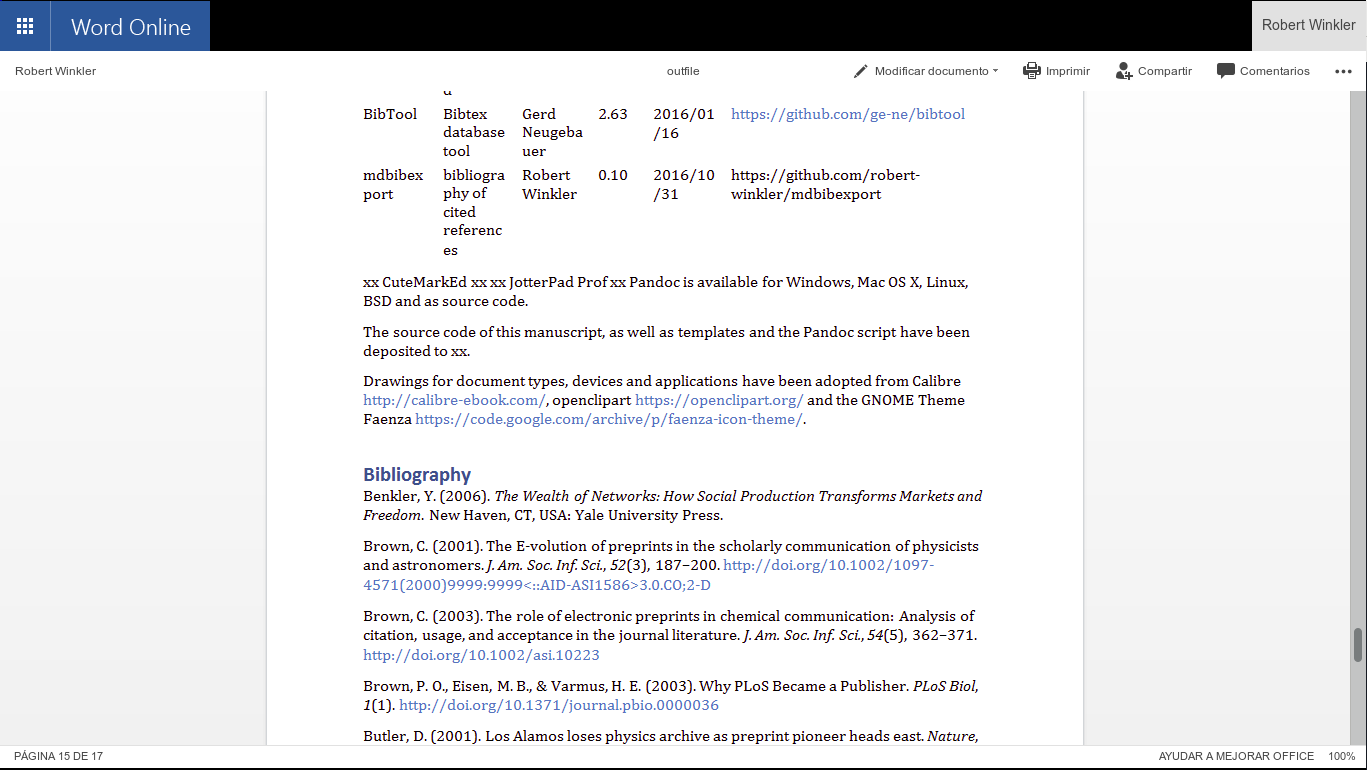
\includegraphics{fig-DOCX-document-in-O365.png}
\caption{Opening a pandoc-generated DOCX in Microsoft Office 365.}
\end{figure}

The same procedure can be applied with an ODT formatted document.

\subsection{Development of a TEX/PDF
template}\label{development-of-a-texpdf-template}

The default pandoc LATEX template can be written into a separate file
by:

\begin{Shaded}
\begin{Highlighting}[]
\KeywordTok{pandoc} \NormalTok{-D latex }\KeywordTok{>} \NormalTok{template-peerj.latex}
\end{Highlighting}
\end{Shaded}

This template can be adjusted, e.g.~by defining Unicode encoding (see
above), by including particular packages or setting document options
(line numbering, font size). The template can then be used with the
pandoc parameter \texttt{-\/-template=pandoc-peerj.latex}.

The templates used for this document are included as Supplemental
Material (see section \emph{Software and code availability} below).

\subsection{Styles for HTML and EPUB}\label{styles-for-html-and-epub}

The style for HTML and EPUB formats can be defined in .css stylesheets.
The Supplemental Material contains a simple example .css file for
modifying the HTML output, which can be used with the pandoc parameter
\texttt{-c\ pandoc.css}.

\section{Automating document
production}\label{automating-document-production}

The commands necessary to produce the document in a specific formats or
styles can be defined in a simple \texttt{Makefile}. An example
\texttt{Makefile} is included in the source code of this preprint. The
desired output file format can be chosen when calling \texttt{make}.
E.g. \texttt{make\ outfile.pdf} produces this preprint in PDF format.
Calling \texttt{make} without any option creates all listed document
types. A \texttt{Makefile} producing DOCX, ODT, JATS, PDF, LATEX, HTML
and EPUB files of this document is provided as Supplemental Material.

\subsection{Cross-platform
compatibility}\label{cross-platform-compatibility}

The \texttt{make} process was tested on Windows 10 and Linux 64 bit. All
documents -- DOCX, ODT, JATS, LATEX, PDF, EPUB and HTML -- were
generated successfully, which demonstrates the cross-platform
compatibility of the workflow.

\section{Perspective}\label{perspective}

Following the trend to peer production, the formatting of scientific
content must become more efficient. Markdown/ pandoc has the potential
to play a key role in the transition from proprietary to
community-driven academic production. Important research tools, such as
the statistical computing and graphics language R (R Core Team, 2014)
and the Jupyter notebook project (Kluyver et al., 2016) have already
adopted the MD syntax (e.g. \url{http://rmarkdown.rstudio.com/}). The
software for writing manuscripts in MD is mature enough to be used by
academic writers. Therefore, publishers also should consider
implementing the MD format into their editorial platforms.

\section{Conclusions}\label{conclusions}

Authoring scientific manuscripts in markdown (MD) format is
straight-forward, and manual formatting is reduced to a minimum. The
simple syntax of MD facilitates document editing and collaborative
writing. The rapid conversion of MD to multiple formats such as DOCX,
LATEX, PDF, EPUB and HTML can be done easily using pandoc, and templates
enable the automated generation of documents according to specific
journal styles.

The additional features we implemented facilitate the correct indexing
of meta information of journal articles according to the `semantic web'
philosophy.

Altogether, the MD format supports the agile writing and fast production
of scientific literature. The associated time and cost reduction
especially favours community-driven publication strategies.

\section{Acknowledgments}\label{acknowledgments}

We cordially thank Dr.~Gerd Neugebauer for his help in creating a subset
of a bibtex data base using BibTool, as well as Dr.~Ricardo A. Chávez
Montes, Prof.~Magnus Palmblad and Martin Fenner for comments on the
manuscript. Warm thanks also go to Anubhav Kumar and Jennifer König for
proofreading. The work was funded by the Consejo Nacional de Ciencia y
Tecnología (CONACyT) Mexico, with the grant FRONTERAS 2015-2/814 and by
institutional funding of the Centro de Investigación y de Estudios
Avanzados del Instituto Politécnico Nacional (CINVESTAV).

\newpage

\section{Software and code
availability}\label{software-and-code-availability}

The relevant software for creating this manuscript used is cited
according to (Smith, Katz \& Niemeyer, 2016) and listed in \textbf{Tab.
3}. Since unique identifiers are missing for most software projects, we
only refer to the project homepages or software repositories:

\begin{longtable}[c]{@{}llllll@{}}
\caption{Relevant software used for this article.}\tabularnewline
\toprule
\begin{minipage}[b]{0.08\columnwidth}\raggedright\strut
\textbf{Software}
\strut\end{minipage} &
\begin{minipage}[b]{0.20\columnwidth}\raggedright\strut
\textbf{Use}
\strut\end{minipage} &
\begin{minipage}[b]{0.17\columnwidth}\raggedright\strut
\textbf{Authors}
\strut\end{minipage} &
\begin{minipage}[b]{0.06\columnwidth}\raggedright\strut
\textbf{Version}
\strut\end{minipage} &
\begin{minipage}[b]{0.06\columnwidth}\raggedright\strut
\textbf{Release}
\strut\end{minipage} &
\begin{minipage}[b]{0.25\columnwidth}\raggedright\strut
\textbf{Homepage/ repository}
\strut\end{minipage}\tabularnewline
\midrule
\endfirsthead
\toprule
\begin{minipage}[b]{0.08\columnwidth}\raggedright\strut
\textbf{Software}
\strut\end{minipage} &
\begin{minipage}[b]{0.20\columnwidth}\raggedright\strut
\textbf{Use}
\strut\end{minipage} &
\begin{minipage}[b]{0.17\columnwidth}\raggedright\strut
\textbf{Authors}
\strut\end{minipage} &
\begin{minipage}[b]{0.06\columnwidth}\raggedright\strut
\textbf{Version}
\strut\end{minipage} &
\begin{minipage}[b]{0.06\columnwidth}\raggedright\strut
\textbf{Release}
\strut\end{minipage} &
\begin{minipage}[b]{0.25\columnwidth}\raggedright\strut
\textbf{Homepage/ repository}
\strut\end{minipage}\tabularnewline
\midrule
\endhead
\begin{minipage}[t]{0.08\columnwidth}\raggedright\strut
pandoc
\strut\end{minipage} &
\begin{minipage}[t]{0.20\columnwidth}\raggedright\strut
universal markup converter
\strut\end{minipage} &
\begin{minipage}[t]{0.17\columnwidth}\raggedright\strut
John MacFarlane
\strut\end{minipage} &
\begin{minipage}[t]{0.06\columnwidth}\raggedright\strut
1.16.0.2
\strut\end{minipage} &
\begin{minipage}[t]{0.06\columnwidth}\raggedright\strut
16/01/13
\strut\end{minipage} &
\begin{minipage}[t]{0.25\columnwidth}\raggedright\strut
\url{http://www.pandoc.org}
\strut\end{minipage}\tabularnewline
\begin{minipage}[t]{0.08\columnwidth}\raggedright\strut
pandoc-citeproc
\strut\end{minipage} &
\begin{minipage}[t]{0.20\columnwidth}\raggedright\strut
library for CSL citations with pandoc
\strut\end{minipage} &
\begin{minipage}[t]{0.17\columnwidth}\raggedright\strut
John MacFarlane, Andrea Rossato
\strut\end{minipage} &
\begin{minipage}[t]{0.06\columnwidth}\raggedright\strut
0.9.1
\strut\end{minipage} &
\begin{minipage}[t]{0.06\columnwidth}\raggedright\strut
16/03/19
\strut\end{minipage} &
\begin{minipage}[t]{0.25\columnwidth}\raggedright\strut
\url{https://github.com/jgm/pandoc-citeproc}
\strut\end{minipage}\tabularnewline
\begin{minipage}[t]{0.08\columnwidth}\raggedright\strut
pandoc-jats
\strut\end{minipage} &
\begin{minipage}[t]{0.20\columnwidth}\raggedright\strut
creation of JATS files with pandoc
\strut\end{minipage} &
\begin{minipage}[t]{0.17\columnwidth}\raggedright\strut
Martin Fenner
\strut\end{minipage} &
\begin{minipage}[t]{0.06\columnwidth}\raggedright\strut
0.9
\strut\end{minipage} &
\begin{minipage}[t]{0.06\columnwidth}\raggedright\strut
15/04/26
\strut\end{minipage} &
\begin{minipage}[t]{0.25\columnwidth}\raggedright\strut
\url{https://github.com/mfenner/pandoc-jats}
\strut\end{minipage}\tabularnewline
\begin{minipage}[t]{0.08\columnwidth}\raggedright\strut
ownCloud
\strut\end{minipage} &
\begin{minipage}[t]{0.20\columnwidth}\raggedright\strut
personal cloud software
\strut\end{minipage} &
\begin{minipage}[t]{0.17\columnwidth}\raggedright\strut
ownCloud GmbH, Community
\strut\end{minipage} &
\begin{minipage}[t]{0.06\columnwidth}\raggedright\strut
9.1.1
\strut\end{minipage} &
\begin{minipage}[t]{0.06\columnwidth}\raggedright\strut
16/09/20
\strut\end{minipage} &
\begin{minipage}[t]{0.25\columnwidth}\raggedright\strut
\url{https://owncloud.org/}
\strut\end{minipage}\tabularnewline
\begin{minipage}[t]{0.08\columnwidth}\raggedright\strut
Markdown Editor
\strut\end{minipage} &
\begin{minipage}[t]{0.20\columnwidth}\raggedright\strut
plugin for ownCloud
\strut\end{minipage} &
\begin{minipage}[t]{0.17\columnwidth}\raggedright\strut
Robin Appelman
\strut\end{minipage} &
\begin{minipage}[t]{0.06\columnwidth}\raggedright\strut
0.1
\strut\end{minipage} &
\begin{minipage}[t]{0.06\columnwidth}\raggedright\strut
16/03/08
\strut\end{minipage} &
\begin{minipage}[t]{0.25\columnwidth}\raggedright\strut
\url{https://github.com/icewind1991/files_markdown}
\strut\end{minipage}\tabularnewline
\begin{minipage}[t]{0.08\columnwidth}\raggedright\strut
BibTool
\strut\end{minipage} &
\begin{minipage}[t]{0.20\columnwidth}\raggedright\strut
Bibtex database tool
\strut\end{minipage} &
\begin{minipage}[t]{0.17\columnwidth}\raggedright\strut
Gerd Neugebauer
\strut\end{minipage} &
\begin{minipage}[t]{0.06\columnwidth}\raggedright\strut
2.63
\strut\end{minipage} &
\begin{minipage}[t]{0.06\columnwidth}\raggedright\strut
16/01/16
\strut\end{minipage} &
\begin{minipage}[t]{0.25\columnwidth}\raggedright\strut
\url{https://github.com/ge-ne/bibtool}
\strut\end{minipage}\tabularnewline
\bottomrule
\end{longtable}

The software created as part of this article, \emph{pandoc-scholar}, is
suitable for general use and has been published at
\url{https://github.com/pandoc-scholar/pandoc-scholar}, DOI:
\href{https://doi.org/10.5281/zenodo.376761}{10.5281/zenodo.376761}. The
source code of this manuscript, as well as the templates and pandoc
Makefile, have been deposited to
\url{https://github.com/robert-winkler/scientific-articles-markdown/}.

Drawings for document types, devices and applications have been adopted
from Calibre \url{http://calibre-ebook.com/}, openclipart
\url{https://openclipart.org/} and the GNOME Theme Faenza
\url{https://code.google.com/archive/p/faenza-icon-theme/}.

\newpage

\section*{Bibliography}\label{bibliography}
\addcontentsline{toc}{section}{Bibliography}

\hypertarget{refs}{}
\hypertarget{ref-benklerux5fwealthux5f2006}{}
Benkler Y. 2006. \emph{The Wealth of Networks: How Social Production
Transforms Markets and Freedom}. New Haven, CT, USA: Yale University
Press.

\hypertarget{ref-berners-leeux5fpublishingux5f2001}{}
Berners-Lee T., Hendler J. 2001. Publishing on the semantic web.
\emph{Nature} 410:1023--1024. DOI:
\href{https://doi.org/10.1038/35074206}{10.1038/35074206}.

\hypertarget{ref-bourneux5fdatabaseux5f2005}{}
Bourne P. 2005. Will a biological database be different from a
biological journal? \emph{PLOS Computational Biology} 1:e34. DOI:
\href{https://doi.org/10.1371/journal.pcbi.0010034}{10.1371/journal.pcbi.0010034}.

\hypertarget{ref-ODF}{}
Brauer M., Durusau P., Edwards G., Faure D., Magliery T., Vogelheim D.
2005. \emph{Open Document Format for Office Applications (OpenDocument)
v1.0}. OASIS.

\hypertarget{ref-brownux5fe-volutionux5f2001}{}
Brown C. 2001. The E-Volution of Preprints in the Scholarly
Communication of Physicists and Astronomers. \emph{J. Am. Soc. Inf.
Sci.} 52:187--200. DOI:
\href{https://doi.org/10.1002/1097-4571(2000)9999:9999\%3C::AID-ASI1586\%3E3.0.CO;2-D}{10.1002/1097-4571(2000)9999:9999\textless{}::AID-ASI1586\textgreater{}3.0.CO;2-D}.

\hypertarget{ref-brownux5froleux5f2003}{}
Brown C. 2003. The Role of Electronic Preprints in Chemical
Communication: Analysis of Citation, Usage, and Acceptance in the
Journal Literature. \emph{J. Am. Soc. Inf. Sci.} 54:362--371. DOI:
\href{https://doi.org/10.1002/asi.10223}{10.1002/asi.10223}.

\hypertarget{ref-brownux5fwhyux5f2003}{}
Brown PO., Eisen MB., Varmus HE. 2003. Why PLoS Became a Publisher.
\emph{PLoS Biol} 1. DOI:
\href{https://doi.org/10.1371/journal.pbio.0000036}{10.1371/journal.pbio.0000036}.

\hypertarget{ref-butlerux5falamosux5f2001}{}
Butler D. 2001. Los Alamos Loses Physics Archive as Preprint Pioneer
Heads East. \emph{Nature} 412:3--4. DOI:
\href{https://doi.org/10.1038/35083708}{10.1038/35083708}.

\hypertarget{ref-callawayux5fpreprintsux5f2013}{}
Callaway E. 2013. Preprints Come to Life. \emph{Nature News} 503:180.
DOI: \href{https://doi.org/10.1038/503180a}{10.1038/503180a}.

\hypertarget{ref-garnetux5fsemiautomaticux5f2015}{}
Corbí A., Burgos D. 2015. Semi-Automated Correction Tools for
Mathematics-Based Exercises in MOOC Environments. \emph{International
Journal of Interactive Multimedia and Artificial Intelligence} 3:89--95.
DOI:
\href{https://doi.org/10.9781/ijimai.2015.3312}{10.9781/ijimai.2015.3312}.

\hypertarget{ref-dominiciux5fpandocux5f2014}{}
Dominici M. 2014. An overview of Pandoc. \emph{TUGboat} 35:44--50.

\hypertarget{ref-dptcollectiveux5ftoolkitux5f2015}{}
DPT Collective. 2015. From Print to Ebooks: A Hybrid Publishing Toolkit
for the Arts. In: Monk J, Rasch M, Cramer F, Wu A eds. Institute of
Network Cultures,

\hypertarget{ref-eikebrokkux5fepubux5f2014}{}
Eikebrokk T., Dahl TA., Kessel S. 2014. EPUB as Publication Format in
Open Access Journals: Tools and Workflow. \emph{Code4Lib}.

\hypertarget{ref-eisenux5fpublishux5f2003}{}
Eisen M. 2003. Publish and be praised. \emph{The Guardian}.

\hypertarget{ref-fecherux5fopenux5f2014}{}
Fecher B., Friesike S. 2014. Open Science: One Term, Five Schools of
Thought. In: Bartling S, Friesike S eds. \emph{Opening Science}.
Springer International Publishing, 17--47.

\hypertarget{ref-ginspargux5ffirstux5f1994}{}
Ginsparg P. 1994. First Steps Towards Electronic Research Communication.
\emph{Computers in Physics} 8:390--396. DOI:
\href{https://doi.org/10.1063/1.4823313}{10.1063/1.4823313}.

\hypertarget{ref-haakux5forcidux5f2012}{}
Haak LL., Fenner M., Paglione L., Pentz E., Ratner H. 2012. ORCID: A
system to uniquely identify researchers. \emph{Learned Publishing}
25:259--264. DOI:
\href{https://doi.org/10.1087/20120404}{10.1087/20120404}.

\hypertarget{ref-HTML5}{}
Hickson I., Berjon R., Faulkner S., Leithead T., Navara ED., O'Connor
E., Pfeiffer S., Faulkner S., Navara ED., Leithead T., Berjon R.,
Hickson I., Pfeiffer S., O'Connor T. 2014. \emph{HTML5}. W3C.

\hypertarget{ref-houghtonux5feconomicux5f2009}{}
Houghton J., Rasmussen B., Sheehan P., Oppenheim C., Morris A., Creaser
C., Greenwood H., Summers M., Gourlay A. 2009. Economic implications of
alternative scholarly publishing models: Exploring the costs and
benefits.

\hypertarget{ref-internationalux5forganizationux5fforux5fstandardizationux5fisoux5f2013}{}
International Organization for Standardization. 2013. ISO 32000-1:2008 -
Document management -- Portable document format -- Part 1: PDF 1.7.
\emph{ISO}.

\hypertarget{ref-internationalux5forganizationux5fforux5fstandardizationux5fisoux2fiecux5f2014}{}
International Organization for Standardization. 2014. ISO/IEC 10646:2014
- Information technology -- Universal Coded Character Set (UCS).
\emph{ISO}.

\hypertarget{ref-kielhornux5fmultiux5f2011}{}
Kielhorn A. 2011. Multi-target publishing-Generating ePub, PDF, and
more, from Markdown using pandoc. \emph{TUGboat-TeX Users Group} 32:272.

\hypertarget{ref-kluyverux5fjupyterux5f2016}{}
Kluyver T., Ragan-Kelley B., Pérez F., Granger B., Bussonnier M.,
Frederic J., Kelley K., Hamrick J., Grout J., Corlay S., others. 2016.
Jupyter notebooks---a publishing format for reproducible computational
workflows. In: \emph{Positioning and power in academic publishing:
Players, agents and agendas}. 87--90. DOI:
\href{https://doi.org/10.3233/978-1-61499-649-1-87}{10.3233/978-1-61499-649-1-87}.

\hypertarget{ref-lamportux5flatex:ux5f1994}{}
Lamport L. 1994. \emph{LaTeX: A Document Preparation System}. Reading,
Mass: Addison-Wesley Professional.

\hypertarget{ref-lanthalerux5fjsonldux5f2012}{}
Lanthaler M., Gütl C. 2012. On using JSON-LD to create evolvable RESTful
services. In: \emph{Proceedings of the third international workshop on
RESTful design}. ACM, 25--32.

\hypertarget{ref-rfc7764}{}
Leonard S. 2016. \emph{Guidance on Markdown: Design Philosophies,
Stability Strategies, and Select Registrations}. RFC Editor; Internet
Request for Comments.

\hypertarget{ref-JATS}{}
National Information Standards Organization. 2012. \emph{JATS: Journal
Article Tag Suite}.

\hypertarget{ref-OOXML}{}
Ngo T. 2006. \emph{OFFICE OPEN XML OVERVIEW ECMA TC45}. Ecma
International.

\hypertarget{ref-ovadiaux5fmarkdownux5f2014}{}
Ovadia S. 2014. Markdown for Librarians and Academics. \emph{Behavioral
\& Social Sciences Librarian} 33:120--124. DOI:
\href{https://doi.org/10.1080/01639269.2014.904696}{10.1080/01639269.2014.904696}.

\hypertarget{ref-Rux5f2014}{}
R Core Team. 2014. \emph{R: A language and environment for statistical
computing}. Vienna, Austria: R Foundation for Statistical Computing.

\hypertarget{ref-HTML4}{}
Raggett D., Hors AL., Jacobs I., Le Hors A., Raggett D., Jacobs I. 1999.
\emph{HTML 4.01 Specification}. W3C.

\hypertarget{ref-shottonux5fcitoux5f2010}{}
Shotton D. 2010. CiTO, the Citation Typing Ontology. \emph{Journal of
Biomedical Semantics} 1:S6. DOI:
\href{https://doi.org/10.1186/2041-1480-1-S1-S6}{10.1186/2041-1480-1-S1-S6}.

\hypertarget{ref-rfc1345}{}
Simonsen K. 1992. \emph{Character Mnemonics \& Character Sets}. Rationel
Almen Planlaegning; Internet Request for Comments.

\hypertarget{ref-smithux5fsoftwareux5f2016}{}
Smith AM., Katz DS., Niemeyer KE. 2016. Software Citation Principles.
\emph{PeerJ Computer Science} 2:e86. DOI:
\href{https://doi.org/10.7717/peerj-cs.86}{10.7717/peerj-cs.86}.

\hypertarget{ref-solomonux5farticleux5f2016}{}
Solomon D., Björk B-C. 2016. Article Processing Charges for Open Access
Publicationthe Situation for Research Intensive Universities in the USA
and Canada. \emph{PeerJ} 4:e2264. DOI:
\href{https://doi.org/10.7717/peerj.2264}{10.7717/peerj.2264}.

\hypertarget{ref-suberux5fopenux5f2012}{}
Suber P. 2012. \emph{Open Access}. Cambridge, Mass: The MIT Press.

\hypertarget{ref-towbinux5felectrophoreticux5f1979}{}
Towbin H., Staehelin T., Gordon J. 1979. Electrophoretic transfer of
proteins from polyacrylamide gels to nitrocellulose sheets: Procedure
and some applications. \emph{Proceedings of the National Academy of
Sciences} 76:4350--4354.

\hypertarget{ref-vanux5fnoordenux5fjournalux5f2012}{}
Van Noorden R. 2012. Journal Offers Flat Fee for ``all You Can
Publish''. \emph{Nature News} 486:166. DOI:
\href{https://doi.org/10.1038/486166a}{10.1038/486166a}.

\hypertarget{ref-vanux5fnoordenux5fopenux5f2013}{}
Van Noorden R. 2013. Open Access: The True Cost of Science Publishing.
\emph{Nature} 495:426--429. DOI:
\href{https://doi.org/10.1038/495426a}{10.1038/495426a}.

\hypertarget{ref-vanux5fnoordenux5farxivux5f2014}{}
Van Noorden R. 2014. The arXiv Preprint Server Hits 1 Million Articles.
\emph{Nature News}. DOI:
\href{https://doi.org/10.1038/nature.2014.16643}{10.1038/nature.2014.16643}.

\hypertarget{ref-volmerux5fhowux5f2016}{}
Volmer DA., Stokes CS. 2016. How to Prepare a Manuscript Fit-for-Purpose
for Submission and Avoid Getting a ``desk-Reject''. \emph{Rapid Commun.
Mass Spectrom.}:n/a--n/a. DOI:
\href{https://doi.org/10.1002/rcm.7746}{10.1002/rcm.7746}.

\hypertarget{ref-willinskyux5funacknowledgedux5f2005}{}
Willinsky J. 2005. The Unacknowledged Convergence of Open Source, Open
Access, and Open Science. \emph{First Monday} 10. DOI:
\href{https://doi.org/10.5210/fm.v10i8.1265}{10.5210/fm.v10i8.1265}.

\hypertarget{ref-woelfleux5fopenux5f2011}{}
Woelfle M., Olliaro P., Todd MH. 2011. Open Science Is a Research
Accelerator. \emph{Nat Chem} 3:745--748. DOI:
\href{https://doi.org/10.1038/nchem.1149}{10.1038/nchem.1149}.

\hypertarget{ref-rfc3629}{}
Yergeau F. 2003. \emph{UTF-8, a transformation format of ISO 10646}.
Alis Technologies.

\hypertarget{ref-youngenux5fcitationux5f1998}{}
Youngen GK. 1998. Citation Patterns to Traditional and Electronic
Preprints in the Published Literature. \emph{Coll. res. libr.}
59:448--456. DOI:
\href{https://doi.org/10.5860/crl.59.5.448}{10.5860/crl.59.5.448}.

\hypertarget{ref-benklerux5fwealthux5f2006}{}
Benkler Y. 2006. \emph{The Wealth of Networks: How Social Production
Transforms Markets and Freedom}. New Haven, CT, USA: Yale University
Press.

\hypertarget{ref-berners-leeux5fpublishingux5f2001}{}
Berners-Lee T., Hendler J. 2001. Publishing on the semantic web.
\emph{Nature} 410:1023--1024. DOI:
\href{https://doi.org/10.1038/35074206}{10.1038/35074206}.

\hypertarget{ref-bourneux5fdatabaseux5f2005}{}
Bourne P. 2005. Will a biological database be different from a
biological journal? \emph{PLOS Computational Biology} 1:e34. DOI:
\href{https://doi.org/10.1371/journal.pcbi.0010034}{10.1371/journal.pcbi.0010034}.

\hypertarget{ref-ODF}{}
Brauer M., Durusau P., Edwards G., Faure D., Magliery T., Vogelheim D.
2005. \emph{Open Document Format for Office Applications (OpenDocument)
v1.0}. OASIS.

\hypertarget{ref-brownux5fe-volutionux5f2001}{}
Brown C. 2001. The E-Volution of Preprints in the Scholarly
Communication of Physicists and Astronomers. \emph{J. Am. Soc. Inf.
Sci.} 52:187--200. DOI:
\href{https://doi.org/10.1002/1097-4571(2000)9999:9999\%3C::AID-ASI1586\%3E3.0.CO;2-D}{10.1002/1097-4571(2000)9999:9999\textless{}::AID-ASI1586\textgreater{}3.0.CO;2-D}.

\hypertarget{ref-brownux5froleux5f2003}{}
Brown C. 2003. The Role of Electronic Preprints in Chemical
Communication: Analysis of Citation, Usage, and Acceptance in the
Journal Literature. \emph{J. Am. Soc. Inf. Sci.} 54:362--371. DOI:
\href{https://doi.org/10.1002/asi.10223}{10.1002/asi.10223}.

\hypertarget{ref-brownux5fwhyux5f2003}{}
Brown PO., Eisen MB., Varmus HE. 2003. Why PLoS Became a Publisher.
\emph{PLoS Biol} 1. DOI:
\href{https://doi.org/10.1371/journal.pbio.0000036}{10.1371/journal.pbio.0000036}.

\hypertarget{ref-butlerux5falamosux5f2001}{}
Butler D. 2001. Los Alamos Loses Physics Archive as Preprint Pioneer
Heads East. \emph{Nature} 412:3--4. DOI:
\href{https://doi.org/10.1038/35083708}{10.1038/35083708}.

\hypertarget{ref-callawayux5fpreprintsux5f2013}{}
Callaway E. 2013. Preprints Come to Life. \emph{Nature News} 503:180.
DOI: \href{https://doi.org/10.1038/503180a}{10.1038/503180a}.

\hypertarget{ref-garnetux5fsemiautomaticux5f2015}{}
Corbí A., Burgos D. 2015. Semi-Automated Correction Tools for
Mathematics-Based Exercises in MOOC Environments. \emph{International
Journal of Interactive Multimedia and Artificial Intelligence} 3:89--95.
DOI:
\href{https://doi.org/10.9781/ijimai.2015.3312}{10.9781/ijimai.2015.3312}.

\hypertarget{ref-dominiciux5fpandocux5f2014}{}
Dominici M. 2014. An overview of Pandoc. \emph{TUGboat} 35:44--50.

\hypertarget{ref-dptcollectiveux5ftoolkitux5f2015}{}
DPT Collective. 2015. From Print to Ebooks: A Hybrid Publishing Toolkit
for the Arts. In: Monk J, Rasch M, Cramer F, Wu A eds. Institute of
Network Cultures,

\hypertarget{ref-eikebrokkux5fepubux5f2014}{}
Eikebrokk T., Dahl TA., Kessel S. 2014. EPUB as Publication Format in
Open Access Journals: Tools and Workflow. \emph{Code4Lib}.

\hypertarget{ref-eisenux5fpublishux5f2003}{}
Eisen M. 2003. Publish and be praised. \emph{The Guardian}.

\hypertarget{ref-fecherux5fopenux5f2014}{}
Fecher B., Friesike S. 2014. Open Science: One Term, Five Schools of
Thought. In: Bartling S, Friesike S eds. \emph{Opening Science}.
Springer International Publishing, 17--47.

\hypertarget{ref-ginspargux5ffirstux5f1994}{}
Ginsparg P. 1994. First Steps Towards Electronic Research Communication.
\emph{Computers in Physics} 8:390--396. DOI:
\href{https://doi.org/10.1063/1.4823313}{10.1063/1.4823313}.

\hypertarget{ref-haakux5forcidux5f2012}{}
Haak LL., Fenner M., Paglione L., Pentz E., Ratner H. 2012. ORCID: A
system to uniquely identify researchers. \emph{Learned Publishing}
25:259--264. DOI:
\href{https://doi.org/10.1087/20120404}{10.1087/20120404}.

\hypertarget{ref-HTML5}{}
Hickson I., Berjon R., Faulkner S., Leithead T., Navara ED., O'Connor
E., Pfeiffer S., Faulkner S., Navara ED., Leithead T., Berjon R.,
Hickson I., Pfeiffer S., O'Connor T. 2014. \emph{HTML5}. W3C.

\hypertarget{ref-houghtonux5feconomicux5f2009}{}
Houghton J., Rasmussen B., Sheehan P., Oppenheim C., Morris A., Creaser
C., Greenwood H., Summers M., Gourlay A. 2009. Economic implications of
alternative scholarly publishing models: Exploring the costs and
benefits.

\hypertarget{ref-internationalux5forganizationux5fforux5fstandardizationux5fisoux5f2013}{}
International Organization for Standardization. 2013. ISO 32000-1:2008 -
Document management -- Portable document format -- Part 1: PDF 1.7.
\emph{ISO}.

\hypertarget{ref-internationalux5forganizationux5fforux5fstandardizationux5fisoux2fiecux5f2014}{}
International Organization for Standardization. 2014. ISO/IEC 10646:2014
- Information technology -- Universal Coded Character Set (UCS).
\emph{ISO}.

\hypertarget{ref-kielhornux5fmultiux5f2011}{}
Kielhorn A. 2011. Multi-target publishing-Generating ePub, PDF, and
more, from Markdown using pandoc. \emph{TUGboat-TeX Users Group} 32:272.

\hypertarget{ref-kluyverux5fjupyterux5f2016}{}
Kluyver T., Ragan-Kelley B., Pérez F., Granger B., Bussonnier M.,
Frederic J., Kelley K., Hamrick J., Grout J., Corlay S., others. 2016.
Jupyter notebooks---a publishing format for reproducible computational
workflows. In: \emph{Positioning and power in academic publishing:
Players, agents and agendas}. 87--90. DOI:
\href{https://doi.org/10.3233/978-1-61499-649-1-87}{10.3233/978-1-61499-649-1-87}.

\hypertarget{ref-lamportux5flatex:ux5f1994}{}
Lamport L. 1994. \emph{LaTeX: A Document Preparation System}. Reading,
Mass: Addison-Wesley Professional.

\hypertarget{ref-lanthalerux5fjsonldux5f2012}{}
Lanthaler M., Gütl C. 2012. On using JSON-LD to create evolvable RESTful
services. In: \emph{Proceedings of the third international workshop on
RESTful design}. ACM, 25--32.

\hypertarget{ref-rfc7764}{}
Leonard S. 2016. \emph{Guidance on Markdown: Design Philosophies,
Stability Strategies, and Select Registrations}. RFC Editor; Internet
Request for Comments.

\hypertarget{ref-JATS}{}
National Information Standards Organization. 2012. \emph{JATS: Journal
Article Tag Suite}.

\hypertarget{ref-OOXML}{}
Ngo T. 2006. \emph{OFFICE OPEN XML OVERVIEW ECMA TC45}. Ecma
International.

\hypertarget{ref-ovadiaux5fmarkdownux5f2014}{}
Ovadia S. 2014. Markdown for Librarians and Academics. \emph{Behavioral
\& Social Sciences Librarian} 33:120--124. DOI:
\href{https://doi.org/10.1080/01639269.2014.904696}{10.1080/01639269.2014.904696}.

\hypertarget{ref-Rux5f2014}{}
R Core Team. 2014. \emph{R: A language and environment for statistical
computing}. Vienna, Austria: R Foundation for Statistical Computing.

\hypertarget{ref-HTML4}{}
Raggett D., Hors AL., Jacobs I., Le Hors A., Raggett D., Jacobs I. 1999.
\emph{HTML 4.01 Specification}. W3C.

\hypertarget{ref-shottonux5fcitoux5f2010}{}
Shotton D. 2010. CiTO, the Citation Typing Ontology. \emph{Journal of
Biomedical Semantics} 1:S6. DOI:
\href{https://doi.org/10.1186/2041-1480-1-S1-S6}{10.1186/2041-1480-1-S1-S6}.

\hypertarget{ref-rfc1345}{}
Simonsen K. 1992. \emph{Character Mnemonics \& Character Sets}. Rationel
Almen Planlaegning; Internet Request for Comments.

\hypertarget{ref-smithux5fsoftwareux5f2016}{}
Smith AM., Katz DS., Niemeyer KE. 2016. Software Citation Principles.
\emph{PeerJ Computer Science} 2:e86. DOI:
\href{https://doi.org/10.7717/peerj-cs.86}{10.7717/peerj-cs.86}.

\hypertarget{ref-solomonux5farticleux5f2016}{}
Solomon D., Björk B-C. 2016. Article Processing Charges for Open Access
Publicationthe Situation for Research Intensive Universities in the USA
and Canada. \emph{PeerJ} 4:e2264. DOI:
\href{https://doi.org/10.7717/peerj.2264}{10.7717/peerj.2264}.

\hypertarget{ref-suberux5fopenux5f2012}{}
Suber P. 2012. \emph{Open Access}. Cambridge, Mass: The MIT Press.

\hypertarget{ref-towbinux5felectrophoreticux5f1979}{}
Towbin H., Staehelin T., Gordon J. 1979. Electrophoretic transfer of
proteins from polyacrylamide gels to nitrocellulose sheets: Procedure
and some applications. \emph{Proceedings of the National Academy of
Sciences} 76:4350--4354.

\hypertarget{ref-vanux5fnoordenux5fjournalux5f2012}{}
Van Noorden R. 2012. Journal Offers Flat Fee for ``all You Can
Publish''. \emph{Nature News} 486:166. DOI:
\href{https://doi.org/10.1038/486166a}{10.1038/486166a}.

\hypertarget{ref-vanux5fnoordenux5fopenux5f2013}{}
Van Noorden R. 2013. Open Access: The True Cost of Science Publishing.
\emph{Nature} 495:426--429. DOI:
\href{https://doi.org/10.1038/495426a}{10.1038/495426a}.

\hypertarget{ref-vanux5fnoordenux5farxivux5f2014}{}
Van Noorden R. 2014. The arXiv Preprint Server Hits 1 Million Articles.
\emph{Nature News}. DOI:
\href{https://doi.org/10.1038/nature.2014.16643}{10.1038/nature.2014.16643}.

\hypertarget{ref-volmerux5fhowux5f2016}{}
Volmer DA., Stokes CS. 2016. How to Prepare a Manuscript Fit-for-Purpose
for Submission and Avoid Getting a ``desk-Reject''. \emph{Rapid Commun.
Mass Spectrom.}:n/a--n/a. DOI:
\href{https://doi.org/10.1002/rcm.7746}{10.1002/rcm.7746}.

\hypertarget{ref-willinskyux5funacknowledgedux5f2005}{}
Willinsky J. 2005. The Unacknowledged Convergence of Open Source, Open
Access, and Open Science. \emph{First Monday} 10. DOI:
\href{https://doi.org/10.5210/fm.v10i8.1265}{10.5210/fm.v10i8.1265}.

\hypertarget{ref-woelfleux5fopenux5f2011}{}
Woelfle M., Olliaro P., Todd MH. 2011. Open Science Is a Research
Accelerator. \emph{Nat Chem} 3:745--748. DOI:
\href{https://doi.org/10.1038/nchem.1149}{10.1038/nchem.1149}.

\hypertarget{ref-rfc3629}{}
Yergeau F. 2003. \emph{UTF-8, a transformation format of ISO 10646}.
Alis Technologies.

\hypertarget{ref-youngenux5fcitationux5f1998}{}
Youngen GK. 1998. Citation Patterns to Traditional and Electronic
Preprints in the Published Literature. \emph{Coll. res. libr.}
59:448--456. DOI:
\href{https://doi.org/10.5860/crl.59.5.448}{10.5860/crl.59.5.448}.

\end{document}
